\chapter{实验几何}\label{chp:experiment_geometry}
几何学是研究“空间”的形体和性质的科学。“空间”就是我们和万物以至星象天体共存的所在。在日常生活中,我们举目四望所见到的地方,都是空间的一部分。同学们在小学数学课中学过的柱体、锥体、球体等等,它们都各自占有空间的一部分,并且构成不同的形体。各种形体的种种性质,如各部分的长度、角度、面积,以及体积等等。都是在我们的生活和生产实践中所不可缺少的知识。
\begin{figure}
	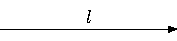
\includegraphics{1-1.pdf}
	\caption{}\label{fig:1-1}
\end{figure}

自古以来,人们经过实践、观察、分析,已总结出一系列的有关空间方面的知识,例如,从中国、埃及、巴比伦、玛雅等古文明中,可以看出对空间的知识都已掌握得相当丰富了。对于空间知识有系统的研究,从西方的古文明中可知,起始于古埃及和巴比伦,而在古希腊得到蓬勃的发展,获得较辉煌的成就。大体说来,古希腊在空间知识方面的成就,由欧几里得集其大成于他所著的《几何原本》\footnote{欧几里得(Euclid,约公元前 300 年左右)所著此书原名 \textit{Elements}, 我国明代数学家徐光启(公元 1562--1633)把书中部分几何内容	译成中文定名为“几何原本”。“几何学”这个中文的名称即来源于此。}这部书中。在这部书里,欧几里得把当时所知道的几何知识经过整理,建立起一个初步完整的理论体系,使这部书反映出几何学是一门偏重于推理、论证的高度理论性的科学。但是,和任何其它科学一样,几何学的理论基础也是建立在实验所得的一些基本事实之上的。在这一章里,我们就通过实验、观察、归纳来研究所得到的知识,为以后进一步学习论证几何作准备。

\section{点、直线和平面}
点、直线和平面是空间最简单的,也是最基本的图形。同学们在日常生活中,对它们早已有直观的认识了。在这一节里,我们再对它们的本质和相互关系作进一步的分析,确立点、直线和平面这三个基本的几何概念,并总结点、直线和平面之间相互关系方面的一些基本性质。

\subsection{点和直线}
在空间,最原始的,也是最基本的概念就是“位置”。通常,我们就用“点”来标记“位置”。例如在一张地图上,我们就以小圆点来标记各地的位置(见\cref{fig:1-2})。
\begin{figure}
	\begin{minipage}[b]{0.48\linewidth}
		\centering
		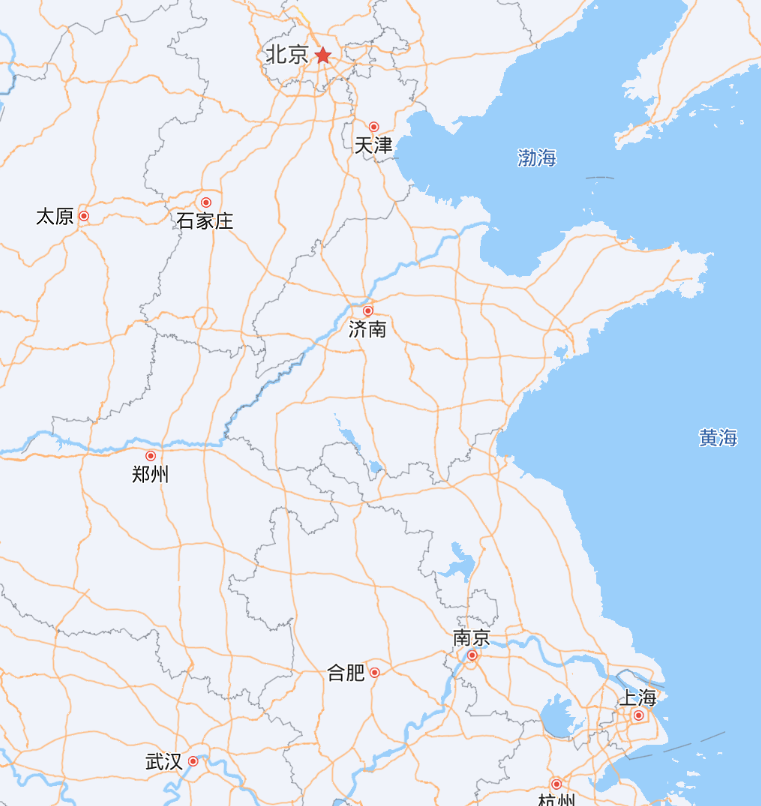
\includegraphics[width=0.9\linewidth]{1-2.png}
		\caption{}\label{fig:1-2}
	\end{minipage}
	\begin{minipage}[b]{0.48\linewidth}
		\centering
		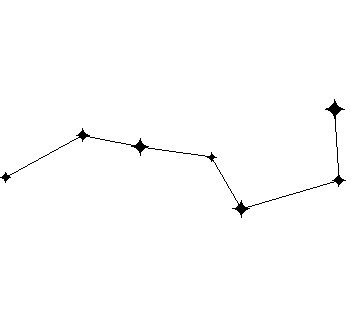
\includegraphics{1-3.pdf}
		\caption{}\label{fig:1-3}
	\end{minipage}
\end{figure}
你可能发现,在地图上北京用“$\star$”,南京用“{$\scriptstyle\odot$}”印制的,这只是为了把首都和地方城市区别开来。其实,北京、南京的“位置”与地图上印制的图形“$\star$”或“{$\scriptstyle\odot$}”的形状和大小是没有关系的。这样,仅仅考虑“位置”的图形就是点。在天象图上也是以小圆点来标记各星体的位置的(见\cref{fig:1-3})。

在几何学的讨论中,我们用不同的大写字母 $A,B,C,\ldots$ 表示不同的点,如\cref{fig:1-4} 中的五个点,就在点旁分别标记以 $A$、$B$、$C$、$D$、$E$,并分别读作点 $A$、点 $B$、点 $C$、点 $D$、点 $E$。

\begin{figure}
  \begin{minipage}[b]{0.48\linewidth}
    \centering
		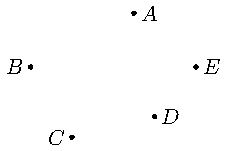
\includegraphics{1-4.pdf}
    \caption{}\label{fig:1-4}
  \end{minipage}
  \begin{minipage}[b]{0.48\linewidth}
    \centering
    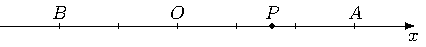
\includegraphics{1-5.pdf}
    \caption{}\label{fig:1-5}
  \end{minipage}
\end{figure}


在日常生活中,我们经常需要从一个地方走到另一个地方。例如,同学们早起上学,就得由自己的家所在的位置走到学校所在的位置。因此,在空间第二个原始的基本概念就要算是“通路”了。所谓“通路”,就是从一个位置移到另一个位置的路线。通常在地图上,我们用线来标记各地之间的种种通路,如铁路、公路等。在几何学的讨论中,“线”就是表示通路的。它的直观含义就是:一个“动点”由一个位置移动到另一个位置所走过的“路线”。如\cref{fig:1-5} 所示,设 $A$、$B$ 两点分别表示空间的两个位置,那么连结 $A$、$B$ 两点的可能通路是很多很多的。

在通常情况下,大家都希望所要走的通路愈短愈好,所以很自然的问题就是:

“在所有连结 $A$、$B$ 两点的各种通路中,哪一条通路最短?”

光线的存在,直截了当地显示给我们下述空间的基本性质:

“连结 $A$、$B$ 两点的最短通路唯一存在,它就是连结 $A$、$B$ 两点的\Concept{直线段}”(在均匀介质中,光走直线\footnote{由光学实验,我们知道光线其实走着最省时间的通路,而并不是走着最短的通路,再者,光的速度是随着“介质”而定的,例如在真空中走的最快,在空气中速度则稍慢(愈稀薄则其速度愈近于真空者),在水中则速度更慢,因为通常我们总是在均匀介质中观察光线,所以光线的速度是个不变的常数。这样,最省时间的通路也就是最短的通路。这就是我们常见常用的事实:光线在均匀介质中走直线。})。

\begin{figure}
	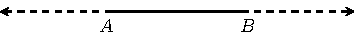
\includegraphics{1-6.pdf}
	\caption{}\label{fig:1-6}
\end{figure}


如\cref{fig:1-6} 所示,由 $A$ 点射向 $B$ 点的光线可以由 $A$ 向 $B$ 的方
向无限延伸;而由 $B$ 点射向 $A$ 点的光线也可以由 $B$ 向 $A$ 的方向无限延伸,所以对于空间任意两点 $A$、$B$,不但存在着唯一的最短通路“直线段 $AB$”,而且也唯一地确定了一条把直线段 $AB$ 两端无限延长的直线,这条直线就叫做由 $A$、$B$ 两点所确定的\Concept{直线},通常称为“直线 $AB$”,而直线段 $AB$ 是直线 $AB$ 介于 $A$、$B$ 两点之间的那一段。

归纳上面的讨论,我们可以作出如下的总结:

\begin{enumerate}[series=conclusion]
	\item “位置”和“通路”是两个最原始的空间概念。在几何学中,以点表示位置,以线表示通路。
	\item 对于任何两点 $A$、$B$,在所有连结、$AB$ 的可能通路中,存在唯一的最短通路,就是连结 $A$、$B$ 两点的直线段。
\end{enumerate}

直线段 $AB$ 也简称线段 $AB$,以后我们用符号 $\overline{AB}$ 表示线段
$AB$。点 $A$,点 $B$ 叫做线段 $AB$ 的\Concept{端点}。有时,一条线段也可以
用一个小写字母来表示,例如线段 $a$、线段 $b$ 等(\cref{fig:1-7a})。

\begin{figure}
	\begin{minipage}[b]{0.4\linewidth}\centering
		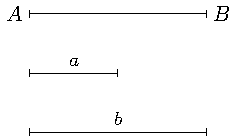
\includegraphics{1-7a.pdf}
		\subcaption{}\label{fig:1-7a}
	\end{minipage}
	\begin{minipage}[b]{0.4\linewidth}\centering
		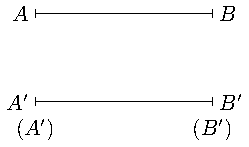
\includegraphics{1-7b.pdf}
		\subcaption{}\label{fig:1-7b}
	\end{minipage}
	\par\smallskip
	\begin{minipage}[b]{0.4\linewidth}\centering
		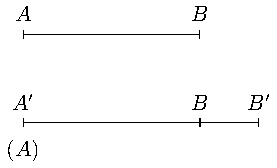
\includegraphics{1-7c.pdf}
		\subcaption{}\label{fig:1-7c}
	\end{minipage}
	\begin{minipage}[b]{0.4\linewidth}\centering
		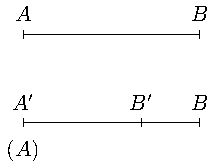
\includegraphics{1-7d.pdf}
		\subcaption{}\label{fig:1-7d}
	\end{minipage}
	\caption{}\label{fig:1-7}
\end{figure}

把 $\overline{AB}$ 放在 $\overline{A'B'}$ 上面,使点 $A$ 和点 $A'$ 重合,$\overline{AB}$ 沿着 $\overline{A'B'}$ 方向落下,那么有以下三种可能情况:
\begin{enumerate}[1)]
	\item 点 $B$ 和点 $B'$ 重合,这时 $\overline{AB}=\overline{A'B'}$ (\cref{fig:1-7b});
	\item 点 $B$ 落在 $A'$ 和 $B'$ 之间,这时 $\overline{AB}<\overline{A'B'}$ (\cref{fig:1-7c});
	\item 点 $B$ 落在 $\overline{A'B'}$ 的延长线上,这时 $\overline{AB}>\overline{A'B'}$(\cref{fig:1-7d})。
\end{enumerate} 

有一根拉直的绳子 $\overline{AB}$,如果把它分成长度相等的两段。但是不许用尺来量,应怎么办?

同学们一定会想到,把绳子 $\overline{AB}$ 的两端点 $A$、$B$ 重叠在一起,并且把绳子拉直,那么在绳子的中间就折出一个 $C$ 点来(\cref{fig:1-8a}), 而被折成的两段绳子 $\overline{AC}$ 和 $\overline{CB}$ 恰好长度相等,这就是说 $C$ 点把 $\overline{AB}$ 平分了。所以我们把平分线段的点叫做\Concept{线段的中点}。如果点 $C$ 是 $\overline{AB}$ 的中点,则 $\overline{AB}=2\overline{AC}=2\overline{CB}$。

\begin{figure}
  \begin{minipage}[b]{0.48\linewidth}
    \centering
		\begin{minipage}{0.5\linewidth}\raggedleft
		  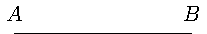
\includegraphics{1-8a.pdf}
		\end{minipage}%
		\begin{minipage}{0.1\linewidth}
		  \subcaption{}\label{fig:1-8a}
		\end{minipage}
		\par\bigskip
		\begin{minipage}{0.5\linewidth}\raggedleft
		  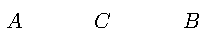
\includegraphics{1-8b.pdf}
		\end{minipage}%
		\begin{minipage}{0.1\linewidth}
		  \subcaption{}\label{fig:1-8b}
		\end{minipage}
    \caption{}\label{fig:1-8}
	\end{minipage}
	\begin{minipage}[b]{0.48\linewidth}
    \centering
		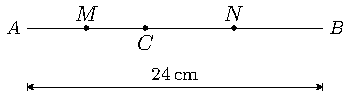
\includegraphics{1-9.pdf}
    \caption{}\label{fig:1-9}
  \end{minipage}
\end{figure}

\begin{example}\label{exp:half_length}
	已知 $\overline{AB}=\qty{24}{cm}$,点 $C$ 在 $\overline{AB}$ 上,点 $M$、$N$ 分别是 $\overline{AC}$ 和 $\overline{CB}$ 的中点,求 $\overline{MN}$ 的长度(见\cref{fig:1-9})。
\end{example}

\begin{solution}
\[\begin{split}
	\overline{MN}&=\overline{MC}+\overline{CN}=\frac{1}{2}\overline{AC}+\frac{1}{2}\overline{CB}\\
	&=\frac{1}{2}\left(\overline{AC}+\overline{CB}\right)=\frac{1}{2}\overline{AB}=\qty{12}{cm}
\end{split}\]
\end{solution}

\begin{enumerate}[resume=conclusion]%\setcounter{enumi}{2} 
	\item 线段可以向两端无限延长,这样就得到一条直线。一条直线可以用表示它上面任	意两点的大写字母来表示,如直线 $CD$。有时为了简便,也可以在这条直线旁标以一个小写字母,如 $\ell$,表示成直线 $\ell$(\cref{fig:1-10})。
	\begin{figure}
		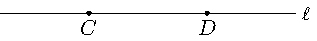
\includegraphics{1-10.pdf}
		\caption{}\label{fig:1-10}
	\end{figure}
	\item 对于任何两点 $A$、$B$,都存在着唯一一条通过 $A$、$B$ 的直线。这个性质就简述为:\emph{两点确定一条直线}。
\end{enumerate}

根据上述性质,我们可以说明其它有关的性质和问题。

\begin{example}
	如果两条直线 $\ell$ 和 $m$ 有一个公共点(交点)$A$(\cref{fig:1-11}),它们还能有其它的公共点吗?为什么?
\end{example}

\begin{figure}
	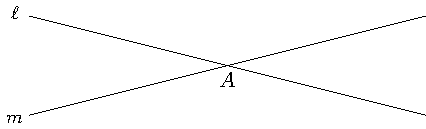
\includegraphics{1-11.pdf}
	\caption{}\label{fig:1-11}
\end{figure}

\begin{solution}
除 $A$ 点外,直线 $\ell$ 和 $m$ 不能再有其它的公共点了。

因为,如果还有另一个公共点 $B$,那么,$\ell$ 和 $m$ 就都是通过 $A$、$B$ 两点的直线。但是通过 $A$、$B$ 两点只有唯一的一条直线,于是,$\ell$ 和 $m$ 就是通过 $A$、$B$ 两点的那条唯一的直线,它们就不是两条不同的直线了。所以,它们除了 $A$ 点外,不可能再有其它的公共点了。

这件事实可以简述为:\emph{两条相交直线确定一交点}。
\end{solution}


\begin{example}
	\cref{fig:1-12} 表示人和物之间放一隔板,使人不能直接看到物的示意图,$A$ 表示物,$E$ 表示人眼,$\overline{BC}$ 表示隔板。为了能看见物的形象,放置一面镜子,图中 $g$ 表示镜面,这时按图1.12(1)中隔板 $\overline{BC}$ 的位置来说,人眼 $E$ 便能看见物 A 的形象,这是为什么?但按图1.12(2)隔板 $\overline{BC}$ 的位置来说,人眼 $E$ 便不能看到物 $A$ 的形象,这又是为什么?
\end{example}

\begin{figure}
	\begin{minipage}[b]{0.45\linewidth}\centering
	  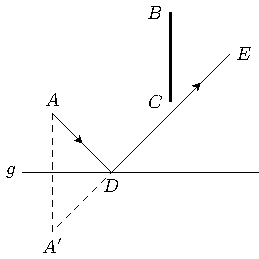
\includegraphics{1-12a.pdf}
		\subcaption{}\label{fig:1-12a}
	\end{minipage}
	\begin{minipage}[b]{0.45\linewidth}\centering
	  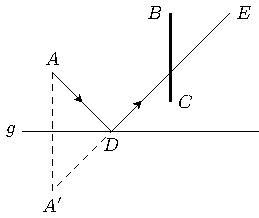
\includegraphics{1-12b.pdf}
		\subcaption{}\label{fig:1-12b}
	\end{minipage}
	\caption{}\label{fig:1-12}
\end{figure}

\begin{solution}
按照镜面映象的道理,人眼 $E$ 是从入射线 $AD$ 和反射线 $DE$ 看见 $A$ 的形象的,而点 $D$ 是点 $E$ 和点 $A$ 的象 $A'$ 的连线 $EA'$ 和 $g$ 的交点,所以 $A$ 的象 $A'$ 是沿着直线 $A'E$ 映入人眼 $E$ 的。因为通过 $A'$ 和 $E$ 只有唯一的一条直线,于是 $A'E$ 和隔板 $\overline{BC}$ 不交(\cref{fig:1-12a})时,在 $E$ 处就看得见 $A$ 的象 $A'$;$A'E$ 和 $\overline{BC}$ 相交,也就是被隔板 $\overline{BC}$ 挡住(\cref{fig:1-12b})时,在 $E$ 处便看不见 $A$ 的象 $A'$ 了。
\end{solution}

\begin{example}\label{exp:segment_count}
如果在已知$\overline{AB}$上依次取 99 个点($C_1,C_2,C_3,\ldots,C_{99}$),那么$\overline{AB}$ 上一共有多少条以这些点为端点的线段?($\overline{AB}$ 也计算在内)
\end{example}	

\begin{solution}
我们分以下几步来研究这个问题:
\begin{enumerate}[leftmargin=2.0em,label=第\chinese*步,font=\bfseries]
	\item 先进行观察、实验。因为每两个点就确定一条线段。因此,
	\begin{enumerate}[leftmargin=0.0em,label=\arabic*)]
    \item 在 $\overline{AB}$ 上取一个点 $C_1$ 时,我们看到\cref{fig:1-13a} 中共有 3 条线段 $\overline{AB}$、$\overline{AC_1}$ 和 $\overline{C_1B}$。
    \begin{figure}
			\begin{minipage}[b]{0.7\linewidth}\centering
				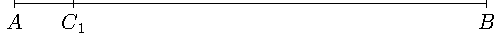
\includegraphics{1-13a.pdf}
			\end{minipage}%
			\begin{minipage}[b]{0.1\linewidth}
				\subcaption{}\label{fig:1-13a}
			\end{minipage}
			\begin{minipage}[b]{0.7\linewidth}\centering
				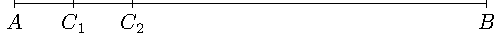
\includegraphics{1-13b.pdf}
			\end{minipage}%
			\begin{minipage}[b]{0.1\linewidth}
				\subcaption{}\label{fig:1-13b}
			\end{minipage}
			\begin{minipage}[b]{0.7\linewidth}\centering
				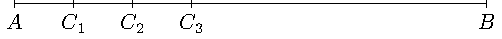
\includegraphics{1-13c.pdf}
			\end{minipage}%
			\begin{minipage}[b]{0.1\linewidth}
				\subcaption{}\label{fig:1-13c}
			\end{minipage}
			\begin{minipage}[b]{0.7\linewidth}\centering
				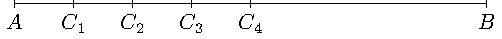
\includegraphics{1-13d.pdf}
			\end{minipage}%
			\begin{minipage}[b]{0.1\linewidth}
				\subcaption{}\label{fig:1-13d}
			\end{minipage}
			\begin{minipage}[b]{0.7\linewidth}\centering
				$\vdots$
			\end{minipage}%
			\begin{minipage}[b]{0.1\linewidth}\centering
				$\vdots$
			\end{minipage}
			\par\smallskip
			\begin{minipage}[b]{0.7\linewidth}\centering
				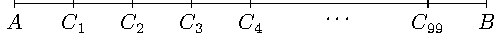
\includegraphics{1-13e.pdf}
			\end{minipage}%
			\begin{minipage}[b]{0.1\linewidth}
				\setcounter{subfigure}{13}
				\subcaption{}\label{fig:1-13e}
			\end{minipage}
			\caption{}\label{fig:1-13}
		\end{figure}
		\item 在 $\overline{AB}$ 上取两个点 $C_1$、$C_2$ 时,我们看到\cref{fig:1-13b} 中共有 6 条线段 $\overline{AB}$、$\overline{AC_1}$、$\overline{C_1B}$、$\overline{AC_2}$、$\overline{C_2B}$ 和 $\overline{C_1C_2}$。
	\item 在 $\overline{AB}$ 上取三个点 $C_1$、$C_2$、$C_3$ 时,我们看到\cref{fig:1-13c} 中有 10 条线段(请同学们自己找出来)。 
	\end{enumerate}
	\item\label{itm:law} 列表分析找规律
	\begin{center}
		\begin{tblr}{colspec={X[c]X[c]},hline{2}=0.8pt}
		$\overline{AB}$ 上取的点数 & $\overline{AB}$ 上线段的总数\\
		1&3\\
		2&6\\
		3&10\\
		$\vdots$&$\vdots$\\
		99& ?\\
		\end{tblr}
	\end{center}

  从表上发现:
	\begin{itemize}
		\item 在 $\overline{AB}$ 上取 1 个点时,$\overline{AB}$ 上的线段总数 $3=1+2$,
		\item 在 $\overline{AB}$ 上取 2 个点时,$\overline{AB}$ 上的线段总数 $6=1+2+3$,
		\item 在 $\overline{AB}$ 上取 3 个点时,$\overline{AB}$ 上的线段总数 $10=1+2+3+4$。
	\end{itemize}

	这时,如果在 $\overline{AB}$上取 4 个点,那么$\overline{AB}$上共有多少条线段呢?由上面发现的规律,可以猜想是 $1+2+3+4+5=15$,数一下\cref{fig:1-13d} 中的线段数,恰好是 15 条。这样自然要问:当在 $\overline{AB}$ 上取 99 个点时,将会有怎样的结果呢?

	\item 归纳、计算

	如果在 $\overline{AB}$上取 99 个点,设这时 $\overline{AB}$ 上的线段总数为 $S$,由在\ref{itm:law}中发现的规律,不难得出:
	\[S=1+2+3+4\cdots +(99+1)=1+2+3+4\cdots +100\]

	这是一个很有趣的计算题,如果按顺序加起来,计算是很麻烦的,我们动动脑筋能否有简便的计算方法呢?

	由于 $S=1+2+3+\cdots +98+99+100$,也就是:
	\[S=100+99+98+\cdots +3+2+1\]

	$\therefore\quad 2S=\underbrace{101+101+101\cdots+101+101+101}_{100\text{项}}=100\times 101$

	$\therefore\quad S=\dfrac{100\times 101}{2}=5050$
\end{enumerate}
\end{solution}

\begin{Practice}
\begin{question}
	\item\label{prac:1-1-1} 图中有几条线段,把它们都写出来。
	\begin{figurehere}
		\begin{minipage}{\linewidth}\centering
			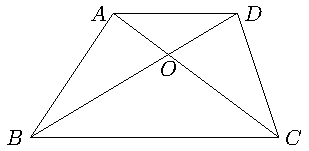
\includegraphics{pr1-1-1.pdf}
			\caption*{第 \ref{prac:1-1-1} 题}
		\end{minipage}
	\end{figurehere}
	\item $A$、$B$、$C$ 三点不在一条直线上,通过其中任何两点画一条直线,一共能画出几条直线?
	\item $A$、$B$、$C$、$D$ 四点中,任何三点都不在一条直线上,通过其中任何两点画一条直线,一共能画出几条直线?
	\item 如果 $A$、$B$、$C$、$D$、$E$ 五点中任何三点都不在一条直线上,通过其中任何两点画一条直线,那么一共能画多少条直线?
	\item 如果有 100 个点,其中任何三点都不在一条直线上,通	过其中任何两点画一条直线,那么一共能画多少条直线?
	\item 工人师付在用方砖铺地时,常常打两个木桩,拉线来铺砖,这样砖就铺得整齐,这是根据了什么道理?
	\item 如果有两个小孩甲、乙在对话,甲问乙:“你的家住在哪里?”乙回答说:“我的家住在直线 $AB$ 的尽头。”试问你能沿着直线 $AB$ 找到乙的家吗?为什么?
	\item 参看\cref{exp:segment_count} 的归纳、计算,如果在 $\overline{AB}$ 上取 $n$ 个点。那么 $\overline{AB}$ 上一共有多少条线段?($\overline{AB}$ 也计算在内)
	\item 已知:$\overline{MN}=\qty{100}{m}$,$P$ 点在 $\overline{MN}$上,$\overline{MP}=\qty{45}{m}$,$S$ 点是 $\overline{PN}$ 的中点,求 $\overline{PS}$的长度是多少米?
	\item 在\cref{exp:half_length} 中,$\overline{MN}$ 的长度与 $C$ 点在 $\overline{AB}$ 上的位置有无关系?
\end{question}
\end{Practice}


\subsection{长度的度量}
在给定两点 $A$、$B$ 之间的所有通路之中,以 $AB$ 为最短,它的“长度”就叫做 $A$、$B$ \Concept{两点间的距离}。所以,两点间的距离是连结这两点的线段的长。

长度是我们经常用的一种几何量,现在让我们分别从实用和数学的观点稍微细致地分析一下“长度”这种几何量的直观含义,并且谈一谈长度的度量。

一般来说,常用的量基本上可以归成两类:其中一类,例如一群羊、一堆蛋,它们具有天然的个别单元,即一只羊、一个蛋。处理这种量,我们只要去数一数它们的“个数”就可以了。因为它们是可数的。用来数“个数”的数学体系就是我们在代数学中一开始就详加讨论的自然数系:$\{1,2,3,\ldots\}$。另一类,例如我们现在要讨论的长度等,这种量虽然不具有天然个别单元,但是,具有一个基本特点:可以无限细分。例如,任给一个线段,不管它怎样短,还是可以把它分割成更短的线段。因此,这种量不可能有天然不可分割的单元,我们处理这种量的办法就是度量。

因为长度这种量并不具有天然不可分割的单位,所以,我们只好选用人为的长度单位。例如“米”就是世界上通用的长度单位。取定长度单位以后,要度量一条线段的长度,也就是要求得它和长度单位之间的“比值”。例如取定长度单位为 \unit{m},所求得的比值是 $1237:1000$,就说这条线段的长度是 \qty{1.237}{m}。但是在实践中,这个比值是怎样求出来的呢?先举几个简单的实例看一看。

\begin{example}\label{exp:divide_mult}
设长度单位是 $u$,所要度量的线段是 $a$ (\cref{fig:1-14})。线段 $a$ 恰好可以分割成 5 段和 $u$ 等长的线段,那么所求的比值是 5,$a$ 的长度就是 $5u$。

一般地说,如果所要度量的线段 $a$ 恰好可以分割成 $m$ 段和 $u$ 等长的线段,那么所求的比值就是整数 $m$,$a$ 的长度就是 $mu$。
\end{example}

\begin{figure}
  \begin{minipage}[b]{0.48\linewidth}
    \centering
		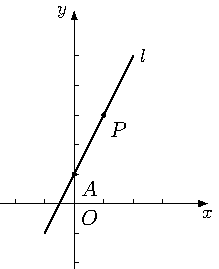
\includegraphics{1-14.pdf}
    \caption{}\label{fig:1-14}
	\end{minipage}
	\begin{minipage}[b]{0.48\linewidth}
    \centering
    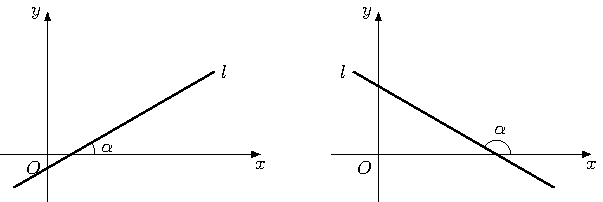
\includegraphics{1-15.pdf}
    \caption{}\label{fig:1-15}
	\end{minipage}
\end{figure}

\begin{example}\label{exp:divide_fraction}
设长度单位是 $u$,所要度量的线段是 $b$(\cref{fig:1-15})单位长 $u$ 恰好可以分割成 3 段和 $b$ 等长的线段,那么所求的比值是 $\dfrac{1}{3}$,$b$ 的长度就是$\dfrac{1}{3}u$。

\bigskip
一般地说,如果长度单位 $u$ 恰好可以分割成 $n$ 段和 $b$ 等长的线段,那么所求的比值是 $\dfrac{1}{n}$,$b$ 的长度就是 $\dfrac{1}{n}u$。
\end{example}

\begin{example}\label{exp:rational_divide}
设长度单位是 $u$,所要度量的线段是 $c$(\cref{fig:1-16})。$c$ 比 $4u$ 长些,但又比 $5u$ 短些,如果我们把 $u$ 三等分,线段$c$截取 4 段 $u$ 后所余的一段恰好是 $\dfrac{1}{3}u$ 的 2 倍,那么$c$ 的长度就是 $4\dfrac{2}{3}u$。

\begin{figure}
	\centering
  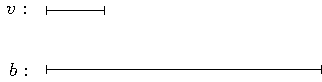
\includegraphics{1-16.pdf}
	\caption{}\label{fig:1-16}
\end{figure}
{\linespread{1.65}\selectfont
一般地说,如果把长度单位 $u$ 适当地等分成 $n$ 段,即每一段 $u'$ 的长度是$\dfrac{1}{n}\cdot u$,所要量的线段 $c$ 恰好可以分割成 $m$ 段和线段 $u'$ 等长的线段,那么 $c$ 的长度就是 $\dfrac{m}{n}u$。

在\cref{exp:rational_divide} 中,用长度单位 $u$ 去度量 $c$ 时,怎样才能知道在 $c$ 上截取 4 段 $u$ 后,所余的一段恰好是 $u$ 的 $\dfrac{1}{3}$ 的整数倍?实际上可以这样来确定:在 $c$ 上截取 4 段 $u$ 后,以所余的一段 $\overline{C_4D}$ 去量 $u$,在 $u$ 上截去一段 $\overline{C_4D}$ 后,所余的一段 $\overline{U_1V}$ 又较 $\overline{C_4D}$ 短,这时再以 $\overline{U_1V}$ 去度量 $\overline{C_4D}$,恰好$\overline{C_4D}$ 是 $\overline{U_1V}$ 的 2 倍。这样便看出 $\overline{U_1V}$ 是 $u$ 的 $\dfrac{1}{3}$,把 $u$ 三等分后,$\overline{C_4D}$ 就恰好是 $\dfrac{1}{3}u$ 的 2 倍了。\par}
\end{example}

\begin{example}\label{exp:rational_divide2}
	设长度单位是 $u$,求线段 $d$ 的长度(\cref{fig:1-17})。
\begin{figure}
	\centering
  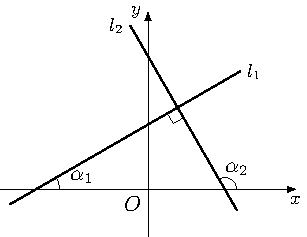
\includegraphics{1-17.pdf}
	\caption{}\label{fig:1-17}
\end{figure}
\end{example}

\begin{solution}
在 $d$ 上用圆规截取 2 段 $u$ 后,所余的一段 $\overline{D_2E}$ 较 $u$ 短;在 $u$ 上截取 2 段 $\overline{D_2E}$ 后,所余的 $\overline{U_2V}$ 较 $\overline{D_2E}$ 短;在 $\overline{D_2E}$ 上截取 2 段 $\overline{U_2V}$ 后,所余的一段 $\overline{F_2E}$ 较 $\overline{U_2V}$ 短;但 $\overline{U_2V}$ 恰好是 $\overline{F_2E}$ 的 2 倍。于是
\[\begin{split}
	\overline{D_2E}&=\overline{D_2F_2}+\overline{F_2E}=2\overline{U_2V}+\overline{F_2E}\\
&=2\cdot 2\overline{F_2E}+\overline{F_2E}=5\overline{F_2E}
\end{split}\]
\[u=2\overline{D_2E}+\overline{U_2V}=2-5\overline{F_2E}+2\overline{F_2E}=12\overline{F_2E}\]
$\therefore\quad \overline{F_2E}=\dfrac{1}{12}u,\quad \overline{D_2E}=\dfrac{5}{12}u,\quad d=2\dfrac{5}{12}u$
\end{solution}

\bigskip
由\cref{exp:rational_divide,exp:rational_divide2} 可以看出,当被度量线段($c$ 和 $d$)不能恰好被分割而成为长度单位的整数倍,也就是它们不能被长度单位量尽时,都是求出另一条线段(\cref{exp:rational_divide} 中是 $\overline{U_1V}$,\cref{exp:rational_divide2} 中是 $\overline{F_2E}$),使得它能量尽长度单位和被量线段。再按\cref{exp:divide_fraction} 的方法求出以长度单位为单位的这条线段的长度,然后便可求出原来被量线段的长度了。

能够量尽两条线段 $a$ 和 $b$ 的线段,我们叫它做线段 $a$ 和 $b$ 的\Concept{公度}。两条线段的公度中最长的,叫做\Concept{这两条线段的最大公度}。$\overline{U_1V}$ 和$\overline{F_2E}$ 就分别是线段 $u$ 和 $c$,$u$ 和 $d$ 的最大公度。在\cref{exp:divide_mult} 中线段$u$ 就是线段 $u$ 和 $a$ 的最大公度;\cref{exp:divide_fraction} 中的线段 $b$ 就是线段 $u$ 和 $b$ 的最大公度,象\cref{exp:rational_divide,exp:rational_divide2} 中求线段 $u$ 和 $c$、$u$ 和 $d$ 的最大公度的方法,叫做\Concept{辗转相截法}。

通过上面各例,我们很自然地会想到:任何两条线段 $a, b$,它们的长度比值是否总是一个分数(整数也可看作分数)?换句话说,对于任何两条线段 $a$、$b$,是否存在着它
们的公度?

这个问题从正、反两面来分析它的重要性。首先,如果任何两条线段的长度的比值总是一个分数,那么分数全体(即代数开始所讲的有理数)就足以处理长度的度量问题了。其次,反过来说,如果两条线段的长度的比值不一定是分数,那么有理数就不足以处理长度的度量问题。因而我们就得学会一种含有“非分数”的数系才能充分解决度量问题。这个问题是整个数学发展史上的一件大事,我们以后再详细讨论。

\begin{Practice}
\begin{question}
	\item 已知线段 $a$、$b$、$u$,其中线段 $a=9u$,$b=3u$,问线段 $a$、$b$ 的最大公度是线段 $u$ 的几倍?
	\item 已知线段 $a=\qty{48}{mm}$,$b=\qty{18}{mm}$。先用辗转相截法求出	$a$、$b$ 的最大公度,并量它等于多少毫米;再用求最大公	约数的辗转相除法求出 48、18 的最大公约数。比较前后所得的结果。
	\item 根据图形填写下面空白:
	\begin{figurehere}
		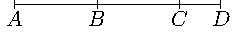
\includegraphics{pr1-2-3.pdf}
	\end{figurehere}
	\begin{tasks}(2)
		\task $\overline{AC}=\overline{BC}+(\qquad)$	
		\task	$\overline{CD}=\overline{AD}-(\qquad)$	
		\task $\overline{AC}+\overline{CD}=(\qquad)+\overline{BD}$
	\end{tasks}
\end{question}
\end{Practice}

\subsection{直线和平面}
在空间,另一种常见的形象就是各种各样的面。例如地球的表面,它的整体看起来是一个略为扁平的球面,而局部的形象又随着当地的地貌而不同。有的地方是一片原,有的地方是起伏的丘陵,有的地方是一片湖面,也有的地方是崇山峻岭和深谷。又如教室的一面墙壁,上课用的黑板,以及桌面等,看起来又都是“平直”的面。

通常检查一个桌面是否“平直”,最简单的方法就是用一根直尺放在桌面上(\cref{fig:1-18}),如果放在任何位置上,直尺的边都和桌面密合,那么桌面就是“平直”的。我们就说桌面是平面。但是象\cref{fig:1-19} 的面上,虽然直尺放在  $\ell_1,\ell_2,\ldots,\ell_n$ 等位置时,直尺边和这个面密合,而在 $AB$ 位置上直尺边和面就不密合了。这就是说并不是在任何位置上直尺的边总和这个面密合,这个面不是一个平面,实际上是一个曲面。
\begin{figure}
  \begin{minipage}[b]{0.48\linewidth}
    \centering
		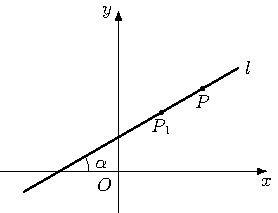
\includegraphics{1-18.pdf}
    \caption{}\label{fig:1-18}
  \end{minipage}
  \begin{minipage}[b]{0.48\linewidth}
    \centering
		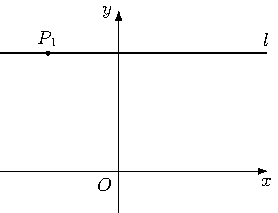
\includegraphics{1-19.pdf}
    \caption{}\label{fig:1-19}
  \end{minipage}
\end{figure}

在几何学的讨论中,平面就是一个到处平直而且向各个方向无限延展的面,它的特点就是在它上面任取两点 $A$ 和 $B$(\cref{fig:1-20}),直线 $AB$ 就完全在这个平面内。

\begin{figure}
  \begin{minipage}[b]{0.48\linewidth}
    \centering
		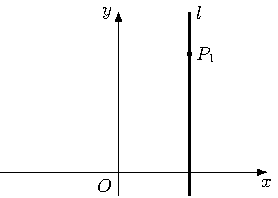
\includegraphics{1-20.pdf}
    \caption{}\label{fig:1-20}
  \end{minipage}
  \begin{minipage}[b]{0.48\linewidth}
    \centering
    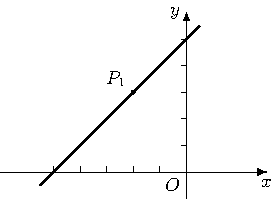
\includegraphics{1-21.pdf}
    \caption{}\label{fig:1-21}
  \end{minipage}
\end{figure}

我们观察一扇门,把它看作平面的一部分,那么它的轴线既在墙壁的平面内(\cref{fig:1-21}),又在这扇门所在的平面内,不可能连结两个“合页”的直线不都在这两个平面内。推动这扇门,它每到一个新的位置都表现了通过轴线的一个平面。这些事实说明了:\emph{空间相交的两个平面的“交界”是一条直线。通过一条直线可有无数个平面。}

\begin{Practice}
\begin{question}
	\item 举出一条直线和一个平面没有公共点的实例,以及一条直线和一个平面只有一个公共点的实例。
	\item 一点在一平面内,而其它的点都不在这个平面内,这种实例有什么?
	\item 举出两个平面没有公共点的实例。
	\item 两个平面只有一个公共点的实例存在吗?
	\item 如果空间被平面 $\alpha$ 分成的两部分之一中,有一只小虫子 $A$,这只小虫子 $A$ 要爬到	被平面所分空间的另一部分去,假如它不穿过平面 $\alpha$,能过去吗?为什么?
\end{question}
\end{Practice}

同学们作这样一个实验,张开手指,使拇指、食指和中指的尖这三点不在一条直线上,拿一张硬纸(它代表一个平面)往三个指尖上放,看看它是否能同时通过三个指尖?再拿一张硬纸仍然这样放,看这两张硬纸是否重合?这种特点对于一个指尖,两个指尖也适合吗?再使母指、食指、中指,无名指的指尖这四点不在一条直线上,看看能否保证总有一张硬纸同时通过这四点?仿照“两点确定一条直线”的特点,同学们能否总结出几个点确定一个平面的结论?

通过上面的实验,我们得出平面的另一个基本性质:\emph{空间不共线三点确定一个平面。}

同学们还可进一步思考以下的问题:
\begin{enumerate}
	\item 一直线及直线外一点能确定一个平面吗?
	\item 相交的两条直线能确定一个平面吗?
\end{enumerate}

\begin{Exercise}
% \addcontentsline{toc}{subsection}{习题1.1}
\begin{question}
	\item 什么是线段?什么是直线?两者有什么区别?
	\item 什么是线段的中点?如果有一根笔直的铁棍,假如用 $\overline{AB}$ 来表示它,不用尺量,也不许把它折弯,你有没有办法找出 $\overline{AB}$ 所表示的这根铁棍的中点来?
% 	\item 请同学们复习一下小学学过的公制、市制两种长度单位,
% 	并填下表:
% 	\begin{center}
% \begin{tabular}{ll}
% 	1公里(km)$=\underline{\qquad}$米(m) &\qquad 1里$=\underline{\qquad}$丈\\
% 1米(m)$=\underline{\qquad}$分米(dm)&\qquad 1丈$=\underline{\qquad}$尺\\
% 1分米(dm)$=\underline{\qquad}$厘米(cm)&\qquad 1尺$=\underline{\qquad}$寸\\
% 1厘米(cm)$=\underline{\qquad}$毫米(mm)&\qquad 1寸$=\underline{\qquad}$分
% \end{tabular}		
% 	\end{center}

% 	\item 	求出下列结果,并化成括号中指定的长度单位:
% \begin{tasks}
% \task 5尺4寸5分 $+$ 3尺4寸 $+$ 6尺7寸8分$=\underline{\qquad}$(米);
% \task 46厘米 $+$ 1米60厘米 $+$ 7米50厘米$=\underline{\qquad}$(尺);
% \task 4丈5尺6寸$\times3=\underline{\qquad}$(米);
% \task 5米40厘米$\div 1000=\underline{\qquad}$(毫米);
% \task 20mm$\times0.1\%=\underline{\qquad}$(m)
% \end{tasks}

\item\label{exec:1-1-3} 在一条直线上,顺次取 $A$、$B$、$C$ 三点,使 $\overline{AB}=\qty{4}{cm}$,$\overline{BC}=\qty{2}{cm}$,并且取 $\overline{AC}$ 的中点 $O$,求:
	\begin{tasks}(3)
		\task $\overline{AO}$ 的长
		\task $\overline{OB}$ 的长
		\task $\overline{OC}$ 的长
	\end{tasks}

\begin{figurehere}
	\begin{minipage}{\linewidth}\centering
		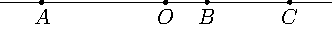
\includegraphics{ex1-1-3.pdf}
		\caption*{第 \ref{exec:1-1-3} 题}
	\end{minipage}
\end{figurehere}

\item 把一条 \qty{32}{cm} 的线段分成三段,中间的一段长为 \qty{8}{cm},问第一段中点到第二段中点的距离等于多少 \unit{cm}?
\item\label{exec:1-1-5} 图中表明四个点可以确定一条、四条或者六条直线。试划图说明五个点可以确定 1、5、6、8 或 10 条直线(其它情况不存在)。
\begin{figurehere}
	\begin{minipage}{\linewidth}\centering
		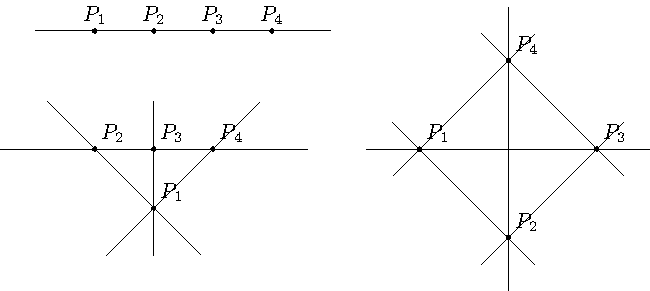
\includegraphics{ex1-1-5.pdf}
		\caption*{第 \ref{exec:1-1-5} 题}
	\end{minipage}
\end{figurehere}

\item\label{exec:1-1-6} 在三角形 $ABC$ 的 $\overline{BC}$ 边上如果取 $n$ 个点$P_1,P_2,P_3,\ldots,P_n$,并把这 $n$ 个点分别和 $A$ 点连结起来,就出现很多三角形,试研究三角形的总数有多少?(原来的三角形 $ABC$ 也包括在内)。

(提示:$\overline{BC}$ 上每一条线段都可与 $A$ 点构成一个三角形,因此求三角形的总数实际上就是求$\overline{BC}$上线段的总数)。
\begin{figurehere}
	\begin{minipage}{\linewidth}\centering
		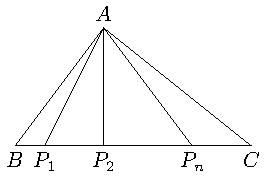
\includegraphics{ex1-1-6.pdf}
		\caption*{第 \ref{exec:1-1-6} 题}
	\end{minipage}
\end{figurehere}
\end{question}
\end{Exercise}

\section{方向、角度与平行}
\subsection{方向与角}
当我们在平坦的操场上要从一个位置(以 $A$ 点表示)走到另一个位置(以 $B$ 点表示),经验告诉我们最省事的走法是:“由 $A$ 点朝向 $B$ 点一直走”。(\cref{fig:1-22})

\begin{figure}
	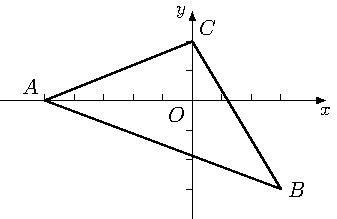
\includegraphics{1-22.pdf}
	\caption{}\label{fig:1-22}
\end{figure}

上面这种常用的走法,很明显地突出了“方向”这个常用的基本几何概念。再设想我们是正在茫茫大海中航行的船的舵手,或者是一架越洋飞行的飞机的驾驶员,那么“方向”这个概念就更是至关紧要的了!因为“航行的方向”是我们随时要确切掌握的要素!

现在让我们就上面的实例,对于所涉及的“方向”这个概念的直观含义,稍加分析。

假如我们从操场的 $A$ 点走向 $B$ 点去(\cref{fig:1-23}),最省事的“通路”当然就是 $\overline{AB}$(因为它是最短的通路)。所以我们先站在 $A$ 点,向 $B$ 点望一望,头脑中抽象地计画了所要走的路线应该是直线段(图中虚线所示)。然后便一步步地沿着设想的路线 $\overline{AB}$ 向 $B$ 点一直走。从几何的观点看,每跨一步就沿着某一个方向做了一个和自己步幅等长的“有向线段”。所以说,“由 $A$ 点朝向 $B$ 点一直走的走法”就是每一步都是沿着 $\overline{AB}$ 这个固定的方向走的那种走法。


\begin{figure}
	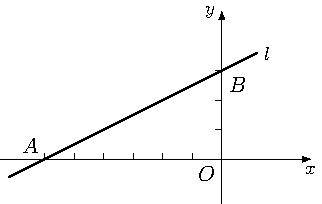
\includegraphics{1-23.pdf}
	\caption{}\label{fig:1-23}
\end{figure}

在由 $A$ 点可以直接看到 $B$ 点的情形下,要保持每一步的方向都是正对着 $B$ 点的方向是很简单的。因为我们随时可以用目光把行进中的位置(\cref{fig:1-23} 中的 $P_n$ 点)和 $B$ 点连一条直线,这条直线的方向也就是下一步(\cref{fig:1-23} 中的 $P_nP_{n+1}$)所要走的方向。但是在另外两个设想的航海和飞行的实例中,目的地是遥远而看不到的,而计划中要走的航线,所经过的绝大部分都是“漫无边际”的海洋和天空,毫无可供“瞄准”的标志。所以要随时保持航行的方向的正确性就变成确保安全到达目的地的最重要的依据了。

由 $A$ 点出发,沿着一个固定的方向(比如向着 $B$ 点的方向)前进时,它的路线就是一条\Concept{射线}。如\cref{fig:1-24} 所示,它就是居于 $A$ 点右侧的那条半直线。
\begin{figure}
  \begin{minipage}[b]{0.48\linewidth}
    \centering
		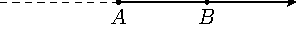
\includegraphics{1-24.pdf}
    \caption{}\label{fig:1-24}
  \end{minipage}
  \begin{minipage}[b]{0.48\linewidth}
    \centering
    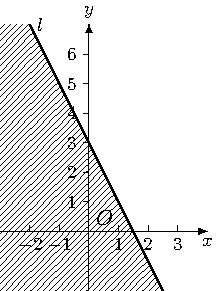
\includegraphics{1-25.pdf}
    \caption{}\label{fig:1-25}
  \end{minipage}
\end{figure}

所以我们把直线上一点一旁的部分叫做\Concept{射线},这一点叫做射线的\Concept{端点}。例如射线 $AB$(\cref{fig:1-24})。(注意:表示射线时,射线的端点字母必须写在前面)。在几何中,我们把以 $A$ 点为端点的一条射线看作是由 $A$ 点出发的一个方向。

我们把从同一端点引出的两条射线所组成的图形叫做\Concept{角},这个共同的端点叫做角的\Concept{顶点},这两条射线分别叫做角的\Concept{边}。我们把角看成是由构成这个角的两条射线所表示的方向差(\cref{fig:1-25})。

一个角通常用符号“$\angle$”(读作角)后边带三个大写字母来表示,中间一个字母表示角的顶点,两旁的两个字母分别表示角的两边上的任意点,如\cref{fig:1-26a} 中的角可记作 $\angle AOB$,读作“角 $AOB$”。如果用一个点作顶点的角只有一个,这个角也可以只用表示顶点的那个大写字母来表示,如\cref{fig:1-26a}  的 $\angle AOB$ 也可表示为 $\angle O$。有时,为了方便,还可以在角的里面靠近顶点写个数字、或小写希腊字母表示角,如\cref{fig:1-26b,fig:1-26c} 中的 $\angle 1$、$\angle 2$、$\angle 3$ 和 $\angle \alpha$、$\angle \beta$、$\angle \gamma$ 等。

\begin{figure}
	\begin{minipage}[b]{0.32\linewidth}\centering
		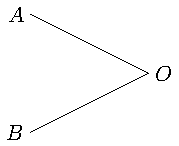
\includegraphics{1-26a.pdf}
		\subcaption{}\label{fig:1-26a}
	\end{minipage}%
	\begin{minipage}[b]{0.32\linewidth}\centering
		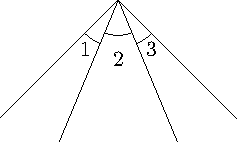
\includegraphics{1-26b.pdf}
		\subcaption{}\label{fig:1-26b}
	\end{minipage}%
	\begin{minipage}[b]{0.32\linewidth}\centering
		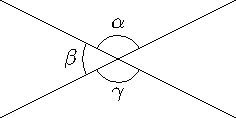
\includegraphics{1-26c.pdf}
		\subcaption{}\label{fig:1-26c}
	\end{minipage}
	\caption{}\label{fig:1-26}
\end{figure}

当一个角的两条边重合时,其夹角显然为 $O$(即方向没有差别)。另外一种特殊情形是当角的一边是另一边的反向延长线时,就称这个角为\Concept{平角}。如\cref{fig:1-27} 中射线 $CA$ 和射线 $CB$ 的方向相反,那么 $\angle ACB$ 就是一个平角。

\begin{figure}
  \begin{minipage}[b]{0.48\linewidth}
    \centering
		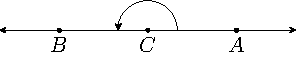
\includegraphics{1-27.pdf}
    \caption{}\label{fig:1-27}
	\end{minipage}
	\begin{minipage}[b]{0.48\linewidth}
    \centering
    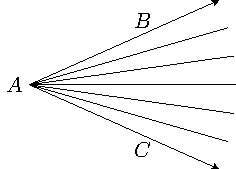
\includegraphics{1-28.pdf}
    \caption{}\label{fig:1-28}
	\end{minipage}
\end{figure}

根据上述,我们可以把日常常用的“方向”和角这两个概念,给以如下的说明:
\begin{enumerate}
	\item 自定点 $A$ 出发的所有方向和以 $A$ 点为端点的所有射线之间一一地相对应。换句话说,对应于自 $A$ 点出发的一个方向,就有唯一的一条射线(它就是自 $A$ 点出发沿着这个固定方向一直走的路线);反之任何一条以 $A$ 点为端点的射线也就唯一地表示了一个确定的方向。所以在几何学中,我们以一条射线表示一个方向。
	\item 一条以 $A$ 为端点的射线,由起始的任何一小段唯一确定(因为整个射线只是那一小段沿着那个方向的无限延伸),所以自 $A$ 点出发的一个方向实可以用它所对应的那条射线开头的任何一小段所表示。
	\item 设射线 $AB$ 和 $AC$ 分别表示由 $A$ 点出发的两个方向,那么 $\angle BAC$ 的直观含义就是射线 $AB$ 和 $AC$ 所表示的那两个方向的差。
	\item 除了零角和平角的特殊情形,如 $A$、$B$、$C$ 三点不共线,我们把射线 $AB$ 由原来的位置沿着平面绕 $A$ 点旋转到射线 $AC$ 的位置所“扫过的区域”叫做 $\angle BAC$ 的\Concept{内部},角的内部也可以叫做\Concept{角区}(\cref{fig:1-28})。
\end{enumerate}

\begin{Practice}
\begin{question}
	\item 什么是射线?射线的直观含义是什么?
	\item 什么是角?角的直观含义是什么?
	\item 线段、射线、直线有什么区别?
	\item\label{prac:1-4-4} 指出图中有几个角?并按图中字母把它们都写出来。
	\item\label{prac:1-4-5} 把图中数字表示的角,改用大写字母表示。
	\item\label{prac:1-4-6} 把图中用小写希腊字母表示的角,改用大写字母表示。
	\begin{figurehere}
		\begin{minipage}[b]{0.25\linewidth}\centering
			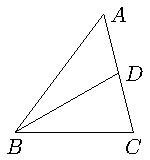
\includegraphics{pr1-4-4.pdf}
			\caption*{第 \ref{prac:1-4-4} 题}
		\end{minipage}%
		\begin{minipage}[b]{0.32\linewidth}\centering
			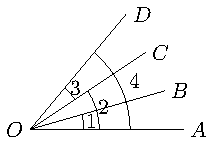
\includegraphics{pr1-4-5.pdf}
			\caption*{第 \ref{prac:1-4-5} 题}
		\end{minipage}%
		\begin{minipage}[b]{0.4\linewidth}\centering
			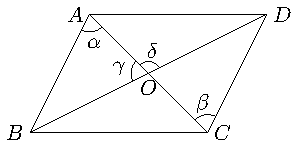
\includegraphics{pr1-4-6.pdf}
			\caption*{第 \ref{prac:1-4-6} 题}
		\end{minipage}
	\end{figurehere}
	\item\label{prac:1-4-7} 指出图中有多少个角,并按图中字母把它们都写出来。
	\item\label{prac:1-4-8} 已知 $P$、$Q$ 两点分别在 $\angle AOB$ 的两边上,试问是否存在不经过 $\angle AOB$ 的内部,由$	P$到$Q$的最短通路?
	\begin{figurehere}
		\begin{minipage}[b]{0.45\linewidth}\centering
		  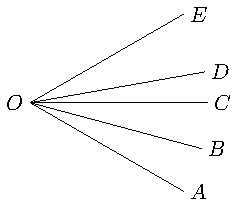
\includegraphics{pr1-4-7.pdf}
			\caption*{第 \ref{prac:1-4-7} 题}
		\end{minipage}%
		\begin{minipage}[b]{0.45\linewidth}\centering
		  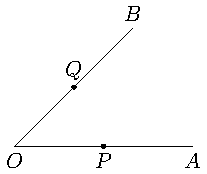
\includegraphics{pr1-4-8.pdf}
			\caption*{第 \ref{prac:1-4-8} 题}
		\end{minipage}
	\end{figurehere}
	\item 如果在射线 $OA$ 上依次取 5 个点,那么在射线 $OA$ 上(包括射线 $OA$ 在内)共有多少条射线?如果依次取 10 个点,100 个点那么在射线 $OA$ 上分别有多少条射线?如果在射线 $OA$ 上取 $n$ 个点,那么在射线 $OA$ 上又有多少条射线?
	\item 如果在直线 $\ell$ 上依次取 3 个点,那么直线 $\ell$ 上有多少条射线?如果取 100 个点,那么直线 $\ell$ 上有多少条射线?如果在 $\ell$ 上依次取 $n$ 个点,那么直线 $\ell$ 上有多少条射线?
\end{question}
\end{Practice}

\subsection{角度和旋转}
在前面我们说明了可以用以 $A$ 点为端点的一条射线来表示一个由 $A$ 点出发的方向。设射线 $AB$ 和 $AC$ 分别表示一个由 $A$ 点出发的两个方向,那么这两条射线所成的角也可以看作是一条以 $A$ 点为端点的射线,从 $AB$ 的位置沿着平面旋转到 $AC$ 的位置而成的图形。象度量线段 $\overline{PQ}$ 的长度就是度量表示 $P$、$Q$ 这两个位置之间的距离一样;度量射线 $AB$ 和 $AC$ 所表示的这两个方向之间的差别也就是度量这两条射线之间所夹的“角度”。而角度也就可以看成是旋转量了。下面采用旋转的观点对于角度的度量再作一初步的探讨:

\subsubsection{角度的大小}
\begin{figure}
	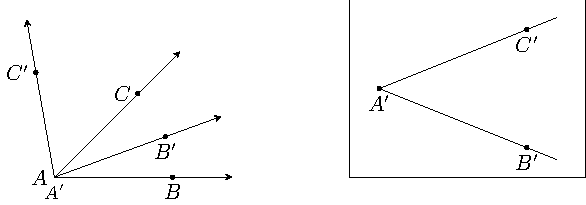
\includegraphics{1-29.pdf}
	\caption{}\label{fig:1-29}
\end{figure}

如\cref{fig:1-29} 所示,$\angle BAC$ 和 $\angle B'A'C'$ 分别是以 $A$ 和 $A'$ 为顶点的两个角,用一张透明的塑胶片,先把它盖在 $\angle B'A'C'$ 的上面,用笔把$\angle B'A'C'$ 复印到塑胶片上。然后把塑胶片移到 $\angle BAC$ 的上面,调整其位置使得顶点 $A$ 和顶点 $A'$ 相重合;再用一个针插在 $A$、$A'$ 点之上,这样,塑胶片仍然可以绕着针尖所插的 $A'$ 点旋转,但是 $A$、$A'$ 点依然确保重合。适当旋转可以使得两个角的边 $AB$ 和 $A'B'$ 重合,而且“角区”位于相重边的同侧(\cref{fig:1-30})。
\begin{figure}
	\begin{minipage}[b]{0.48\linewidth}
    \centering
		\includegraphics{1-30.pdf}
    \caption{}\label{fig:1-30}
  \end{minipage}
  \begin{minipage}[b]{0.48\linewidth}
    \centering
    \includegraphics{1-31.pdf}
    \caption{}\label{fig:1-31}
  \end{minipage}
\end{figure}


这样,两角之间有下列三种可能的位置关系:
\begin{itemize}
	\item 它们的另一边也重合,那么就说这两个角相等,记作 $\angle B'A'C'=\angle BAC$;
	\item $A'C'$ 落在 $\angle BAC$ 的内部,那么就说 $\angle B'A'C'$ 小于 $\angle BAC$,记作 $\angle B'A'C'<\angle BAC$;
	\item $A'C'$ 落在 $\angle BAC$ 的外部,那么就说 $\angle B'A'C'$ 大于 $\angle BAC$,记作 $\angle B'A'C'>\angle BAC$。
\end{itemize}

\subsubsection{两角的相加}
如\cref{fig:1-31} 所示,$\angle BAC$ 和 $\angle CAD$ 两个角的顶点相同,有一条边相重合(即射线 $AC$),而且两者的角区分居于公共边的两侧,就说 $\angle BAD$ 为 $\angle BAC$ 和 $\angle CAD$ 之和,即 $\angle BAD=\angle BAC+\angle CAD$。这时由等式的性质,又可知 $\angle BAC=\angle BAD-\angle CAD$,$\angle CAD=\angle BAD-\angle BAC$。

当两个角相加后是一个平角时,就说这两个角\Concept{互为补角},其中一个角叫做另一个角的补角。简称为\Concept{互补}(\cref{fig:1-32a})。一个角如果和它的补角相等,这个角叫做\Concept{直角}(\cref{fig:1-32b})。

\begin{figure}
	\begin{minipage}[b]{0.45\linewidth}\centering
	  \includegraphics{1-32a.pdf}
		\subcaption{}\label{fig:1-32a}
	\end{minipage}
	\begin{minipage}[b]{0.45\linewidth}\centering
	  \includegraphics{1-32b.pdf}
		\subcaption{}\label{fig:1-32b}
	\end{minipage}
	\caption{}\label{fig:1-32}
\end{figure}

小于直角的角叫做\Concept{锐角},大于直角小于平角的角叫做\Concept{钝角}。如\cref{fig:1-33} 所示,$\angle AOB$ 为锐角,$\angle CPD$ 为钝角。
\begin{figure}
	\begin{minipage}[b]{0.45\linewidth}\centering
		\includegraphics{1-33a.pdf}
		\subcaption{}\label{fig:1-33a}
	\end{minipage}
	\begin{minipage}[b]{0.45\linewidth}\centering
		\includegraphics{1-33b.pdf}
		\subcaption{}\label{fig:1-33b}
	\end{minipage}
	\caption{}\label{fig:1-33}
\end{figure}

如果两个角相加的和等于直角,这两角叫做互为\Concept{余角}。其中一个角叫做另一个角的余角。例如\cref{fig:1-34} 中的 $\angle\alpha+\angle\beta=$ 直角,则$\angle\alpha$、$\angle\beta$ 互为余角。

\begin{figure}
	\includegraphics{1-34.pdf}
	\caption{}\label{fig:1-34}
\end{figure}

\subsubsection{角的度量与量角器}
角的度量和线段的度量的做法基本上是相同的。也是先取定一个角度单位,然后用这个单位,或把它适当等分所得的分单位去和一个要量的角来比较大小。常用的单位是把一个平角分成 180 等份,其中一份叫做 1 度;再把 1 度分成 60 等份,其中一份叫做 1 分;再把 1 分分成 60 等份,其中一份叫做 1 秒。常用的符号是在数字的右上角上标以“\unit{\degree}”表示度,“\unit{\arcminute}”表示分,“\unit{\arcsecond}”表示秒。例如:35 度 12 分 30 秒就写成 \ang{35;12;30}。

平角$=\ang{180}$,平角的二等分角(即平角的一半)就是直角,直角$=\ang{90}$。四个直角相加得一周角,周角$=\ang{360}$。

\begin{figure}
  \includegraphics{1-35.pdf}
	\caption{}\label{fig:1-35}
\end{figure}

度量长度的常用工具是刻有等分刻度的直尺,相应地度量角度的常用工具是\cref{fig:1-35} 所示的量角器。量角器是一个具有 180 个等分刻度的半圆形塑胶板,当我们要去量一个给定的角的角度时,先把顶点和这个半圆板的圆心叠合,然后使得直径和角的一边相重合;那么角的另一边通过半圆的位置的刻度就是所量角度的近似值。如\cref{fig:1-36} 中的 $\angle BAC$,$AB$ 与 \ang{0} 线重合,$AC$ 恰好落在 \ang{40} 的刻度上,所以$\angle BAC=\ang{40}$。

\begin{figure}
	\includegraphics{1-36.pdf}
	\caption{}\label{fig:1-36}
\end{figure}

\begin{example}
	求 \ang{30;19;21} 与 \ang{18;40;42} 的和。
\end{example}

\begin{solution}
\[ \ang{30;19;21}+\ang{18;40;42}=\ang{48;59;63} =\ang{49;;3}\]
\end{solution}

\begin{example}
	把 \ang{3.62} 化成度、分、秒。
\end{example}

\begin{solution}
$\because\quad 1^{\circ}=60',\qquad \therefore\quad 0.62^{\circ}=60'\times 0.62=37.2'$

$\because\quad 1'=60'',\qquad \therefore\quad 0.2'=60''\times 0.2=12''$

$\therefore\quad \ang{3.62}=\ang{3;37;12}$
\end{solution}

\begin{example}
	把 \ang{15;18;15} 化为度。
\end{example}


\begin{solution}
	先把 \ang{;;15} 化为分:
\[\frac{\ang{;;15}}{\ang{;;60}}=\ang{;0.25;}\]
$\therefore\quad \ang{;18;15}=\ang{;18.25;}$。
再把 \ang{;18.25;} 化为度:
\[\frac{\ang{;18.25;}}{\ang{;60;}}\approx \ang{0.304}\]
$\therefore\quad \ang{15;18;15}\approx \ang{15.304}$。
\end{solution}

\subsubsection{对顶角相等和两条直线互相垂直}

如\cref{fig:1-37} 所示 直线 $AB$ 和 $CD$ 相交于 $O$ 点,这时,$\angle AOC$ 和 $\angle BOD$ 中 $OA$ 和 $OB$,$OC$ 和 $OD$ 都互为反向延长线。象这样,一个角的两边分别是另一个角的两边的反向延长线时,我们就称这两个角为\Concept{对顶角}。

\begin{figure}
	\includegraphics{1-37.pdf}
	\caption{}\label{fig:1-37}
\end{figure}

如果两个角是对顶角,那么它们之间有什么关系呢?由\cref{fig:1-37} 可知,$\angle AOC$ 和 $\angle AOD$ 互为补角,即 $\angle AOC+\angle AOD=\ang{180}$;$\angle BOD$ 和 $\angle AOD$ 也互为补角,即 $\angle BOD+\angle AOD=\ang{180}$,因而  $\angle AOC+\angle AOD=\angle BOD+\angle AOD$,所以,$\angle AOC=\angle BOD$。

总结上述事实就成为下述性质:\emph{对顶角相等}。

\begin{example}
如果两条直线 $AB$、$CD$ 相交于 $O$ 点(\cref{fig:1-37}),$\angle AOC=\ang{40}$,求 $\angle BOD$,$\angle AOD$,$\angle COB$ 的度数。
\end{example}

\begin{solution}
两条直线 $AB$、$CD$ 相交于 $O$ 点

$\therefore\quad \angle AOC$ 和 $\angle BOD$ 是对顶角,$\therefore\quad \angle AOC=\angle BOD$(对顶角相等)。

$\because\quad \angle AOC=\ang{40}$

$\therefore\quad \angle BOD=\ang{40}$。

又:$\angle AOC+\angle AOD=\ang{180}$,

$\therefore\quad \angle AOD=\ang{180}-\angle AOC=\ang{180}-\ang{40}=\ang{140}$。

$\because\quad \angle AOD=\angle COB$(对顶角相等)

$\therefore\quad \angle COB=\ang{140}$
\end{solution}

由于两条直线相交得出四个角,根据对顶角的概念可知,这四个角分为两双对顶角,当然每双对顶角都是相等的。并且不难看出,如果两条直线相交得出的四个角中,有一个是直角,那么其余的三个角也都是直角。

\medskip\noindent
\begin{minipage}{0.65\linewidth}\parindent2em
当两条直线相交成直角时,这两条直线就叫做\Concept{互相垂直}。其中一条叫做另一条的垂线,交点叫做\Concept{垂足}。如\cref{fig:1-38} 所示 $\ell_1$ 和 $\ell_2$ 互相垂直,$O$ 是它们的垂足,记作 $\ell_1\perp \ell_2$ 于 $O$ 点。符号“$\perp$”读作“垂直于”。

因为三角板中有一个角是直角,所以可以用三角板来画垂线。
\end{minipage}%
\begin{minipage}{0.35\linewidth}\centering
\begin{figurehere}
  \includegraphics{1-38.pdf}
	\caption{}\label{fig:1-38}
\end{figurehere}
\end{minipage}

\begin{example}
	过已知点 $A$,画已知直线 $\ell$ 的垂线。
\end{example}

\begin{solution}
\begin{enumerate}
	\item $A$ 点在直线 $\ell$ 上
	\item $A$ 点在直线 $\ell$ 外
\end{enumerate}
过 $A$ 点画直线 $\ell$ 的垂线的方法如\cref{fig:1-39} 所示。

\begin{figure}
	\begin{minipage}[b]{0.48\linewidth}
		\centering
		\includegraphics{1-39a.pdf}
		\caption*{过直线 $\ell$ 上一点 $A$ 划 $\ell$ 的垂线}
	\end{minipage}
	\begin{minipage}[b]{0.48\linewidth}
		\centering
		\includegraphics{1-39b.pdf}
		\caption*{过直线 $\ell$ 外一点 $A$ 划 $\ell$ 的垂线}
	\end{minipage}
	\caption{}\label{fig:1-39}
\end{figure}
\end{solution}

\begin{enumerate}[label=问题~\arabic*,leftmargin=1em,font=\bfseries]
	\item 实际画一画,过已知直线上或直线外一点,画这条直线的垂线能画几条?
	\item 如\cref{fig:1-40}, $P$ 点是直线 $AB$ 外一点,$PC\perp AB$ 于 $C$ 点,$D$、$E$ 都是直线 $AB$ 上的点,连结 $\overline{PD}$、$\overline{PE}$,量一量 $\overline{PC}$、$\overline{PD}$、$\overline{PE}$ 哪一条最短?
\end{enumerate}

\medskip
通过上面的实践,我们可以得出垂线的下列性质:
\begin{Theorem}{性质}
	\begin{enumerate}
	\item 过一点作一条直线的垂线,只能作一条。
	\item 从直线外一点和这条直线上各点所引的线段中,垂直线段最短。
\end{enumerate}
\end{Theorem}

\begin{figure}
	\begin{minipage}[b]{0.48\linewidth}
		\centering
		\includegraphics{1-40.pdf}
		\caption{}\label{fig:1-40}
	\end{minipage}
	\begin{minipage}[b]{0.48\linewidth}
		\centering
		\includegraphics{1-41.pdf}
	\caption{}\label{fig:1-41}
	\end{minipage}
\end{figure}

过直线外一点画这条直线的垂线,这点到垂足间的线段的长度叫做这点到这条直线的\Concept{距离}。

例如,从直线 $\ell$ 外一点 $A$,向直线 $\ell$ 画垂线,设垂足为 $B$,那么$\overline{AB}$ 的长度就是点 $A$ 到直线 $\ell$ 的距离(\cref{fig:1-41})。

\subsubsection{三角形的内角和}

我们观察手中的一副三角板(\cref{fig:1-42}),它们的大小形状都不相同;其中一个三角板的三个角和另一个三角板的三个角之间的大小,虽然都有一个直角,但其余的两对角的大小是不一样的,如果我们把每个三角形三个角的大小各自加起来:
\[\begin{split}
\ang{90}+\ang{45}+\ang{45}&=\ang{180}\\
\ang{90}+\ang{60}+\ang{30}&=\ang{180}	
\end{split}\]
结果发现两个三角板的三个角的和都相同,都等于 \ang{180}。

\begin{figure}
  \includegraphics{1-42.pdf}
	\caption{}\label{fig:1-42}
\end{figure}

这样,我们自然地会想到:任何一个三角形的三个角的和等于多少度?是否也等于 \ang{180}?

同学们在纸上任意画两个三角形,形状、大小都不要一样,但要认真仔细地画,边要画得直,笔道要越细越好。然后用量角器去量它们的各角,把每一个三角形的三个角的度数加起来,如果得到的两个结果相差很大,就再仔细地量一量、算一算,如果得到的两个结果相差极为微小,而且都极其接近 \ang{180}, 那么我们又会想到:如果在量的过程中没出现误差,是否任何一个三角形的三个角的和都等于 \ang{180}?

带着这个问题,我们不妨这样来设想,因为 \ang{180} 角即平角,它的两边合成一条直线,如果三角形三个角的大小的和等于 \ang{180},那么这三个角拼合起来就应该得到一个平角。因此我们可以按照这个设想,再来检验三角形三个角的和是否为一个平角,即 \ang{180}角。

先用硬纸板仔细地剪出一个三角形(如\cref{fig:1-43a}),然后在桌上放一把直尺(\cref{fig:1-43a});再沿着\cref{fig:1-43a} 中任意画的虚线把三个角(记作$\angle 1$,$\angle 2$,$\angle 3$)剪下来;最后按\cref{fig:1-43b} 所示,把 $\angle 1$,$\angle 2$,$\angle 3$ 拼合起来放在直尺的边上,结果,作为 $\angle 1$,$\angle 2$,$\angle 3$ 之和的角的两边恰好和直尺的边密合。

\begin{figure}
	\begin{minipage}[b]{0.45\linewidth}\centering
    \includegraphics{1-43a.pdf}
		\subcaption{}\label{fig:1-43a}
	\end{minipage}
	\begin{minipage}[b]{0.45\linewidth}\centering
    \includegraphics{1-43b.pdf}
		\subcaption{}\label{fig:1-43b}
	\end{minipage}
	\caption{}\label{fig:1-43}
\end{figure}

通过以上实践,我们便总结出实验的结果,这就是:

\begin{Theorem}{性质}
三角形的三个角的和是 \ang{180}。	
\end{Theorem}

\begin{example}
已知如\cref{fig:1-44}, $\triangle ABC$ 中,$\angle A=\ang{55}$,$\angle B=\ang{48}$。$BD\perp AC$于 $D $点。求 $\angle DBC$ 的度数。
\end{example}
\par\medskip\noindent
\begin{minipage}{0.7\linewidth}
	\begin{solution}
		$\because\,\,$ 三角形的三个角之和是 \ang{180}
		
		$\therefore\,\, \angle A+\angle ABC+\angle C=\ang{180}$
		
		$\therefore\,\, \angle C=\ang{180}-\angle A-\angle ABC
		=\ang{180}-\ang{55}-\ang{48}=\ang{77}$。
		
		又 $\because\,\, BD\perp AC$ 于 $D$ 点,
		
		$\therefore\,\, \angle BDC=\ang{90} $
		
		$\therefore\,\, \angle DBC=\ang{180}-\angle C-\angle BDC
		=\ang{180}-\ang{77}-\ang{90}=\ang{13}$。
	\end{solution}
\end{minipage}%
\begin{minipage}{0.3\linewidth}\centering
  \begin{figurehere}
		\includegraphics{1-44.pdf}
		\caption{}\label{fig:1-44}
	\end{figurehere}
\end{minipage}

\begin{Practice}
\begin{question}
	\item\label{prac:1-5-1} 看图在各题的(\qquad)中填入适当的角:
	\begin{tasks}(2)
		\task $\angle ABD=\angle ABC+(\qquad )$
		\task $\angle CBE-\angle DBE=(\qquad)$
		\task* $\angle ABE-\angle CBD=\angle ABC+(\qquad)$
	\end{tasks}
	\begin{figurehere}
		\begin{minipage}[b]{0.48\linewidth}
			\centering
			\includegraphics{pr1-5-1.pdf}
			\caption*{第 \ref{prac:1-5-1} 题}
		\end{minipage}
		\begin{minipage}[b]{0.48\linewidth}
			\centering
			\includegraphics{pr1-5-4.pdf}
			\caption*{第 \ref{prac:1-5-4} 题}
		\end{minipage}
	\end{figurehere}
	\item\label{prac:1-5-2} 什么是平角、直角、锐角、钝角?指出下列图中的锐角、直角和钝角。
	\begin{figurehere}
		\begin{minipage}{\linewidth}\centering
			\includegraphics{pr1-5-2.pdf}
			\caption*{第 \ref{prac:1-5-2} 题}
		\end{minipage}
	\end{figurehere}
	\item 分别指出,时针和分针在下列哪个时间组成锐角、钝角、直角和平角。
	\begin{tasks}(3)
		\task 4 点
		\task 6 点
		\task 9 点
		\task 1 点 30 分
		\task 2 点 5分
	\end{tasks}
	\item\label{prac:1-5-4} 什么叫两个角互补?如果已知 $\angle AOB$,试画出 $\angle AOB$ 的补角。
	\item 什么叫两个角互为余角?如果 $\angle \alpha+\angle \beta=$ 直角,那么说“$\angle \alpha$ 是余角”,“$\angle\beta$ 是余角”,对吗?怎样才是正确的说法?
	\item\label{prac:1-5-6} 用量角器分别量出下列各角的度数。
	\begin{figurehere}
		\begin{minipage}{\linewidth}\centering
			\includegraphics{pr1-5-6.pdf}
			\caption*{第 \ref{prac:1-5-6} 题}
		\end{minipage}
	\end{figurehere}
	\item 用量角器分别画出 \ang{45},\ang{72},\ang{90},\ang{134} 的角。
	\item\label{prac:1-5-8} 什么叫对顶角?下列各图中有没有对顶角?如果有,把它们写出来。
	\begin{figurehere}
		\begin{minipage}{\linewidth}
		\begin{minipage}[b]{0.3\linewidth}\centering
			\includegraphics{pr1-5-8a.pdf}
			\subcaption{}
		\end{minipage}%
		\begin{minipage}[b]{0.3\linewidth}\centering
			\includegraphics{pr1-5-8b.pdf}
			\subcaption{}
		\end{minipage}%
		\begin{minipage}[b]{0.4\linewidth}\centering
			\includegraphics{pr1-5-8c.pdf}
			\subcaption{}
		\end{minipage}
		\caption*{第 \ref{prac:1-5-8} 题}
		\end{minipage}
	\end{figurehere}
	\item\label{prac:1-5-9} 已知(如图)直线 $AB$ 和 $CD$ 相交于 $O$ 点,$\angle AOC=\ang{50;20;}$,求 $\angle BOD$、$\angle COB$ 和 $\angle AOD$。
	\item 计算下列各题:
	\begin{tasks}(2)
		\task $\ang{3;25;18}+\ang{24;39;24}$
		\task $\ang{64;27;15}-\ang{28;37;35}$
	\end{tasks}
	\begin{figurehere}
		\begin{minipage}[b]{0.48\linewidth}
			\centering
			\includegraphics{pr1-5-9.pdf}
			\caption*{第 \ref{prac:1-5-9} 题}
		\end{minipage}
		\begin{minipage}[b]{0.48\linewidth}
			\centering
			\includegraphics{pr1-5-16.pdf}
			\caption*{第 \ref{prac:1-5-16} 题}
			\end{minipage}
	\end{figurehere}
	\item 化下列单名数为复名数(度、分、秒)。
	\[1.25^{\circ};\quad 0.8^{\circ};\quad 3.21^{\circ};\quad (1\frac{1}{2})^{\circ};\quad (2\frac{1}{3})^{\circ}\]
	\item 化下列复名数为单名数(度)。
	\[\ang{5;30;};\quad \ang{12;36;12};\quad \ang{38;4;5}\]
	\item 求 \ang{23.26}、\ang{15;25;15} 的角的补角的大小。
	\item 求 \ang{48;15;}、\ang{72.9} 的角的余角的大小。
	\item 什么是两点间的距离?什么是直线外一点到这条直线的距离?
	\item\label{prac:1-5-16} 已知:$P$ 在直线 $\ell$ 上,$Q$ 在直线 $m$ 上,试量出:
	\begin{tasks}(2)
		\task $P$、$Q$ 两点间的距离;
		\task $P$ 到直线 $m$ 的距离;
		\task $Q$ 点到直线 $\ell$ 的距离。
	\end{tasks}
	\item\label{prac:1-5-17} 已知如图,用三角板:
	\begin{tasks}(2)
		\task 过 $A$ 点画出直线 $BC$ 的垂线;
		\task 过 $B$ 点画出直线 $AC$ 的垂线;
		\task 过 $C$ 点画出直线 $AB$ 的垂线。
	\end{tasks}
	\begin{figurehere}
		\begin{minipage}[b]{0.48\linewidth}
			\centering
			\includegraphics{pr1-5-17.pdf}
			\caption*{第 \ref{prac:1-5-17} 题}
		\end{minipage}
		\begin{minipage}[b]{0.48\linewidth}
			\centering
			\includegraphics{pr1-5-19.pdf}
			\caption*{第 \ref{prac:1-5-19} 题}
		\end{minipage}
	\end{figurehere}
	\item 已知$\triangle ABC$中,$\angle A=\ang{70}$, $\angle B=\ang{60}$,求 $\angle C$。
	\item\label{prac:1-5-19} 如图,$\angle 1=\ang{35}$,$\angle 2=\ang{78}$,求 $\angle 3$ 的大小,自 $\angle 3$ 的顶点画一条射线和 $\angle 1$ 的一条边相交,并且使 $\angle 4=\ang{16}$。

	问:$\angle 5$比$\angle 2$少多少度?
	\item 怎样从“三角形三个内角和等于 \ang{180}”推算出四边形的四个内角的和,五边形五个内角的和,六边形六个内角的和各等于多少度?
	\item\label{prac:1-5-21} 如果分别延长 $\triangle ABC$ 的三边 $AB$、$BC$、$CA$ 得到 $\angle 1$、$\angle 2$ 和 $\angle 3$,那么 $\angle 1+\angle 2+\angle 3=?$
	\item\label{prac:1-5-22} 如果顺次延长四边形 $ABCD$ 的各边,得到 $\angle 1$、$\angle 2$、$\angle 3$ 和 $\angle 4$,那么,请你根据第 \ref{prac:1-5-21} 题的计算结果猜想一下这四个角之和可能是多少度?然后再计算一下 $\angle 1+\angle 2+\angle 3+\angle 4=?$ 来验证一下你的猜想是否正确。
	\begin{figurehere}
		\begin{minipage}[b]{0.48\linewidth}
			\centering
			\includegraphics{pr1-5-21.pdf}
			\caption*{第 \ref{prac:1-5-21} 题}
		\end{minipage}
		\begin{minipage}[b]{0.48\linewidth}
			\centering
			\includegraphics{pr1-5-22.pdf}
			\caption*{第 \ref{prac:1-5-22} 题}
			\end{minipage}
	\end{figurehere}
\end{question}
\end{Practice}

\subsection{角度和平行}
在前面的讨论中,我们已经明确了沿着一个固定方向一直走,所经过的路线就是一条射线。如\cref{fig:1-45} 所示,射线 $AB$ 和射线 $A'B'$ 分别表示起点为 $A$ 和 $A'$ 的两个方向。连结 $A$、$A'$ 再延长得射线 $AA'$,于是射线 $AC$ 和射线 $A'C'$ 是相同的两个方向;$\angle CAB$ 表示射线 $AB$ 和 $AC$ 这两个方向的差别,$\angle C'A'B'$ 表示射线 $A'B'$ 和 $A'C'$ 这两个方向的差别。如果 $\angle CAB=\angle C'A'B'$,显然射线 $AB$ 和 $A'B'$ 的方向就是相同的。

\begin{figure}
	\begin{minipage}[b]{0.48\linewidth}
		\centering
    \includegraphics{1-45.pdf}
		\caption{}\label{fig:1-45}
	\end{minipage}
	\begin{minipage}[b]{0.48\linewidth}
		\centering
		\includegraphics{1-46.pdf}
		\caption{}\label{fig:1-46}
	\end{minipage}
\end{figure}


我们把 $\angle CAB$ 和 $\angle C'A'B'$ 这样位置的角叫做\Concept{同位角}。如\cref{fig:1-46} 所示。

连结同一平面内的射线 $AB$ 和 $A'B'$ 的端点 $A$、$A'$ 后,如果得到的同位角相等(\cref{fig:1-45})即 $\angle CAB=\angle C'A'B'$,我们就说射线 $AB$ 和 $A'B'$ 互相平行。同样地,如果同一平面内的两条直线 $\ell$ 和 $\ell'$ 被另一条直线 $AA'$ 截出的同位角相等(\cref{fig:1-47}),我们就说直线 $\ell$ 和 $\ell'$ \Concept{互相平行}。记作 $\ell\parallel \ell'$。

\begin{figure}
    \begin{minipage}[b]{0.48\linewidth}
    	\centering
			\includegraphics{1-47.pdf}
    	\caption{}\label{fig:1-47}
    \end{minipage}
    \begin{minipage}[b]{0.48\linewidth}
    	\centering
			\includegraphics{1-48.pdf}
    \caption{}\label{fig:1-48}
  \end{minipage}
\end{figure}

\begin{example}
在纸上画一条直线记为 $\ell$,在 $\ell$ 外任意取一点 $A'$(\cref{fig:1-48}),怎样在纸上过 $A'$ 画一条直线和 $\ell$ 平行?
\end{example}

\begin{solution}
根据同位角相等,两条直线就平行,这一平行线的意义,我们在直线 $\ell$ 上先取一点$A$,再连结出直线 $AA'$,然后量出 $\angle 1$ 的大小,并用量角器划出 $\angle 2=\angle 1$,这时 $\angle 2$ 的另一条边所在直线 $\ell'$ 就是 $\ell$ 的平行线。如果在 $\ell$ 上另取一点 $B$,仍用画同位角 $\angle 4=\angle 3$ 的方法画出过点$A'$ 和直线 $\ell$ 平行的直线,结果这条直线仍然是 $\ell'$。

同样地,如果在直线 $\ell$ 上另取点 $C$、$D$、……(图中没有画出)而后分别按上面的方法画出过点 $A'$ 和 $\ell$ 的平行线,结果这条直线还是 $\ell'$。

通过画图,我们得到:
\begin{Theorem}{性质}
	过已知直线 $\ell$ 外的一点 $P$ 只有一条直线和 $\ell'$ 平行。
\end{Theorem}
\end{solution}

\begin{example}
	教室里的长方形黑板的对边是不是平行线?为什么(\cref{fig:1-49})?
\end{example}

\smallskip\noindent
\begin{minipage}{0.5\linewidth}\parindent2em
	\begin{solution}
		由小学数学课中我们已知长方形的各角都是直角,如图,长方形的 $\angle 1$、$\angle 2$、$\angle 3$、$\angle 4$ 都是直角。
		
		因为 $\angle 1'$ 是 $\angle 1$ 的补角,所以 $\angle 1'$ 也是直角,于是同位角 $\angle 1'=\angle 2$,因此长方形的对边 $a\parallel a'$。 
		
		同样,同位角 $\angle 3'=\angle 2$,因此另一对边 $b\parallel b'$。 
	\end{solution}
\end{minipage}
\begin{minipage}{0.45\linewidth}\centering
	\begin{figurehere}\quad
		\includegraphics{1-49.pdf}
		\caption{}\label{fig:1-49}
	\end{figurehere}
\end{minipage}

\medskip 
我们学习了平行线的意义之后,进一步考虑平面上两条直线 $\ell$,$m$ 有几种可能的位置关系呢?参看\cref{fig:1-50},同学们自己归纳出结论。
\begin{figure}
	\includegraphics{1-50.pdf}
	\caption{}\label{fig:1-50}
\end{figure}

\begin{Practice}
\begin{question}
	\item\label{prac:1-6-1} 如图,在同一平面内,直线 $m$ 和 $\ell$ 垂直于 $A$ 点,直线 $\ell$ 和 $m$ 垂线于 $A'$ 点,直线 $\ell$ 和 $\ell'$ 平行吗?为什么?
	\item\label{prac:1-6-2} 如图,先把三角板的一边 $a$ 和直线 $\ell$ 密合;再用直尺和三角板的另一边 $b$ 密合;固定直尺,推动三角板使$b$总和直尺密合,当 $a$ 过 $P$ 点时,沿 $a$ 画直线 $\ell'$,那么 $\ell'\parallel \ell$。为什么?
	\begin{figurehere}
		\begin{minipage}[b]{0.48\linewidth}
			\centering
			\includegraphics{pr1-6-1.pdf}
			\caption*{第 \ref{prac:1-6-1} 题}
		\end{minipage}
		\begin{minipage}[b]{0.48\linewidth}
			\centering
			\includegraphics{pr1-6-2.pdf}
			\caption*{第 \ref{prac:1-6-2} 题}
		\end{minipage}
	\end{figurehere}
\item 已知直线 $AB$ 外一点 $C$,过 $C$ 点划一条直线和 $AB$ 平行。
\item 两条平行直线是否可以确定一个平面?
\end{question}
\end{Practice}

\begin{Exercise}
\begin{question}
	\item 用度、分、秒表示下列各角:
	\begin{tasks}(3)
		\task $\dfrac{1}{2}$直角
		\task $\dfrac{1}{4}$直角
		\task $1\dfrac{1}{4}$直角
		\task \ang{48.45}
		\task \ang{58.19}
		\task \ang{;;384600}
	\end{tasks}
	\item 计算下列式子:
	\begin{tasks}(2)
		\task $\ang{38;24;}+\ang{54;43;}$
		\task $\ang{180}-\ang{99;48;}$
		\task $52^{\circ}13'-27^{\circ}58'$
		\task $24^{\circ}3'\times 15$
		\task $200^{\circ}45'\div 5$
		\task $\ang{144}\div \ang{12}$
		\task $\ang{18;33;} \div 4$
		\task $\ang{315;5;}\div \ang{14;8;}$
	\end{tasks}
	\item\label{exec:1-2-3} 检验图中两条直线 $OA$,$O'A'$ 是否平行。
	\begin{figurehere}
		\begin{minipage}[b]{0.48\linewidth}
			\centering
			\includegraphics{ex1-2-3.pdf}
			\caption*{第 \ref{exec:1-2-3} 题}
		\end{minipage}
		\begin{minipage}[b]{0.48\linewidth}
			\centering
			\includegraphics{ex1-2-4.pdf}
			\caption*{第 \ref{exec:1-2-4} 题}
		\end{minipage}
	\end{figurehere}
	\item\label{exec:1-2-4} 检验图中的两条直线是否垂直。
	\item 回答下列问题:
	\begin{tasks}
		\task 钝角与锐角的差一定比直角大吗?举例说明。
		\task 两个锐角的和会不会大于直角?会不会大于或等于平角?
		\task 两个钝角的和会不会大于或等于一个周角。
	\end{tasks}
	\item 下面的说法对不对?为什么?
	\begin{tasks}(2)
		\task 锐角的余角是锐角。
		\task 锐角的补角是锐角。
		\task 直角的补角是直角。
		\task 两个锐角不能互为补角。
		\task! 两个角如果互余,这两个角都是锐角。
		\task! 一个锐角和一个钝角一定互为补角。
		\task! 两个角如果互补,一定是一个角为锐角一个角为钝角。
		\task! 一个锐角加上一个锐角,还是一个锐角。
		\task! 一个钝角减去一个比它小的钝角,差是锐角。
	\end{tasks}
	\item 一个角的补角是它的 3 倍,求这个角的度数。
	\item 一个角的余角是它的 3 倍,求这个角的度数。
	\item 一个角是它的补角的 4 倍,求这个角是多少度?
	\item 两个角的度数比为 $7:2$,它们的差是 \ang{50},求这两个角的度数。
	\item 两条直线相交有一个角是 \ang{20},求其余各角。
	\item\label{exec:1-12} 已知 $AB$ 是直线,$O$ 点在 $AB$ 上,直线 $CO\perp DO$,那么 $\angle 1$ 与$\angle 2$ 互余吗?为什么?
	\item\label{exec:1-13} 如图,试:
	\begin{tasks}(2)
		\task 过 $B$ 点画直线 $AD$ 的垂线?
		\task 过 $D$ 点画直线 $BC$ 的垂线?
		\task 过 $O$ 点画直线 $BD$ 的垂线?
	\end{tasks}
	\begin{figurehere}
		\begin{minipage}[b]{0.48\linewidth}
			\centering
			% \includegraphics{ex1-12.pdf}
			\caption*{第 \ref{exec:1-12} 题}
		\end{minipage}
		\begin{minipage}[b]{0.48\linewidth}
			\centering
			% \includegraphics{ex1-13.pdf}
			\caption*{第 \ref{exec:1-13} 题}
		\end{minipage}
	\end{figurehere}
	\item 下面的说法对不对?说明理由。
	\begin{tasks}
		\task 可能有三个角都是锐角的三角形。
		\task 可能有二个角都是直角的三角形。
		\task 不可能有一个角是直角,另一个角是钝角的三角形。
		\task 可能有一个角是钝角,其余两个角都是锐角的三角形。
	\end{tasks}
\end{question}
\end{Exercise}

\section{全等和叠合}
\subsection{全等形}
两个形状和大小完全相同的图形,叫做全等形。如\cref{fig:1-51a} 中,三角形 \MyRoman{2} 和 \MyRoman{1} 面积的大小相等但形状不同; \MyRoman{3} 和 \MyRoman{1} 的形状相同但大小又不等; \MyRoman{4} 和 \MyRoman{1} 的形状和大小都不一样,只有 \MyRoman{5} 和 \MyRoman{1} 的形状和大小完全相同。三角形 \MyRoman{1} 和 \MyRoman{5} 是全等的。又如\cref{fig:1-51b} 中,三棱锥 \MyRoman{1}$'$ 和 \MyRoman{2}$'$ 形状相同但大小不等;\MyRoman{3}$'$ 和 \MyRoman{2}$'$ 体积的大小相等但形状又不同。只有 \MyRoman{4}$'$ 和 \MyRoman{2}$'$ 的形状和大小完全相同。三棱锥 \MyRoman{2}$'$ 和 \MyRoman{4}$'$ 是全等的。

\begin{figure}
  \begin{minipage}{\linewidth}\centering
		\includegraphics{1-51a.pdf}
		\subcaption{}\label{fig:1-51a}
	\end{minipage}
  \begin{minipage}{\linewidth}\centering
		\includegraphics{1-51b.pdf}
		\subcaption{}\label{fig:1-51b}
	\end{minipage}
	\caption{}\label{fig:1-51}
\end{figure}

我们用符号“$\cong$”表示全等。在图中就有:
\begin{center}
	三角形 \MyRoman{1} $\cong$ 三角形 \MyRoman{5};\qquad 三棱锥 \MyRoman{2}$'\cong$ 三棱锥 \MyRoman{4}$'$
\end{center}

对于平面上两个图形(简称平面图形),要看一看他们是否全等,实践检验的方法,常常是看它能否叠合。能叠合的就全等。

显然,两条线段 $\overline{AB}$ 和 $\overline{A'B'}$ 能叠合的唯一条件就是它们等长:$\overline{AB}=\overline{A'B'}$。

在角的度量的讨论中,我们实际就是用叠合来说明两个角的大小相等的意义的,这也就是说两个角 $\angle A$ 和 $\angle A'$ 能叠合的唯一条件就是它们的大小相等:$\angle A=\angle A'$。

如果 $\triangle ABC$ 和 $\triangle A'B'C'$ 全等(\cref{fig:1-52}),这就是说它们能叠合。因而他们的边和角便分别相等(也说全等形的对应边相等、对应角相等):
\begin{figure}
  \includegraphics{1-52.pdf}
	\caption{}\label{fig:1-52}
\end{figure}
\[\begin{split}
\overline{AB}=\overline{A''C''},&\quad \overline{BC}=\overline{B''C''},\quad \overline{CA}=\overline{B''A''}\\
\angle A=\angle A'',&\quad \angle B=\angle C'',\quad \angle C=\angle B''
\end{split}\]

\subsection{三角形全等的条件}
由上面对两个全等三角形的分析,知道了两个三角形如果全等,它们的对应边、对应角都分别相等。反过来说,如果两个三角形的各边对应相等,对应角也分别相等,那么这两个三角形便能叠合,它们就是全等三角形。

下面我们来研究两个三角形的全等条件。

\begin{enumerate}
	\item 如\cref{fig:1-53} 中,$\angle A=\angle A'$,$\overline{AB}=\overline{A'B'}$,$\overline{AC}=\overline{A'C'}$。那么可以使$\overline{A'B'}$ 叠合在 $\overline{AB}$ 上,从而 $\angle A'$ 可以和 $\angle A$ 叠合,同时 $\overline{A'C'}$ 也就叠合在 $\overline{AC}$ 上了。这样一来,由于点 $B'$ 落在点 $B$ 上,点 $C'$ 落在点 $C$ 上,那么根据“两点只确定一条直线”这个基本性质,直线 $B'C'$ 便叠合在直线 $BC$ 上,自然 $\overline{B'C'}$ 和 $\overline{BC}$ 也就叠合在一起,于是 $\triangle ABC$ 和 $\triangle A'B'C'$ 便完全叠合,它们也就全等了。
	\begin{figure}
		\includegraphics{1-53.pdf}
		\caption{}\label{fig:1-53}
	\end{figure}

	由此可见,检验两个三角形是否全等时,不必分别的检验它们的各边是否对应相等、各对应角是否相等,而是检验出两条边和所夹的角分别相等就可判定这两个三角形全等了。这种判定两个三角形全等的条件,记作(SAS)条件。
	\item 与此相仿,如\cref{fig:1-53} 中 $\angle A=\angle A'$,$\overline{AB}=\overline{A'B'}$,$\angle B=\angle B'$,也可以先使 $\overline{A'B'}$ 叠合在 $\overline{AB}$ 上,再让 $\triangle A'B'C'$ 落在 $\triangle ABC$ 所在平面上,因为 $\angle A'=\angle A$,$\angle B'=\angle B$,所以 $\angle A'$ 和 $\angle A$,$\angle B'$ 和 $\angle B$ 分别叠合;这样,直线 $A'B'$ 和 $AC$,$B'C'$ 和 $BC$ 也就分别叠合了,由于“两条直线相交只有一个交点”。因此,点 $A'$ 必落在点 $A$ 上,于是 $\triangle A'B'C'$ 和 $\triangle ABC$ 就完全叠合了,因此它们全等。这就是说两角和夹边对应相等的两个三角形全等。这种判定两个三角形全等的条件,记作(ASA)条件。
	\item 再有,如果一个三角形的三条边的长度确定了,通过观察和实验我们可以发现这个三角形的形状和大小就不会改变了(\cref{fig:1-54a})。而一个四边形如果四条边的长度确定了,它的形状和大小却是可以改变的(\cref{fig:1-54b})。我们把三角形的这种特性叫做三角形的\Concept{稳定性}。
	\begin{figure}
		\begin{minipage}[b]{0.45\linewidth}\centering
			\includegraphics{1-54a.pdf}
			\subcaption{}\label{fig:1-54a}
		\end{minipage}
		\begin{minipage}[b]{0.45\linewidth}\centering
			\includegraphics{1-54b.pdf}
			\subcaption{}\label{fig:1-54b}
		\end{minipage}
		\caption{}\label{fig:1-54}
	\end{figure}

	这样,一个三角形 $ABC$ 的三边和另一个三角形 $A'B'C'$ 的三边如果对应地相等,即 $\overline{AB}=\overline{A'B'}$,$\overline{BC}=\overline{B'C'}$,$\overline{AC}=\overline{A'C'}$,那么由三角形的稳定性,这两个三角形的对应角也必相等。即 $\angle A=\angle A'$,$\angle B=\angle B'$,$\angle C=\angle C'$。因此,这两个三角形就全等。这种判定三角形全等的条件,记作(SSS)条件。
\end{enumerate}

\begin{example}
  在\cref{fig:1-55} 中,如果已知 $\overline{AB}=\overline{DC}$,$\overline{AC}=\overline{DB}$,$\triangle ABC$ 和 $\triangle DCB$ 全等吗?为什么?
\end{example}

\medskip\noindent
\begin{minipage}{0.6\linewidth}
	\begin{solution}
		在 $\triangle ABC$ 和 $\triangle DCB$ 中,由于:
		\begin{align*}
			\overline{AB}&=\overline{DC}  \tag{已知}\\
			\overline{AC}&=\overline{DB} \tag{已知}\\
			\overline{BC}&=\overline{BC}  \tag{公共边}	
		\end{align*}
		$\therefore\quad \triangle ABC\cong \triangle DCB$(SSS)。
	\end{solution}
\end{minipage}%
\begin{minipage}{0.4\linewidth}\centering
  \begin{figurehere}
		\includegraphics{1-55.pdf}
		\caption{}\label{fig:1-55}
	\end{figurehere}
\end{minipage}

\begin{example}
在\cref{fig:1-56} 中已知 $\overline{AD}=\overline{AE}$,$\overline{AB}=\overline{AC}$,那么 $\triangle ABE$ 和 $\triangle ACD$ 全等吗?为什么?
\end{example}

\noindent
\begin{minipage}{0.6\linewidth}
	\begin{solution}
		在$\triangle ABE$和$\triangle ACD$中,由于:
		\begin{align*}
			\overline{AD}&=\overline{AE}  \tag{已知}\\
			\overline{AB}&=\overline{AC} \tag{已知}\\
			\angle A&=\angle A  \tag{公共角}	
		\end{align*}
	$\therefore\quad \triangle ABE\cong \triangle ACD$(SAS)。
	\end{solution}
\end{minipage}%
\begin{minipage}{0.4\linewidth}\centering
  \begin{figurehere}
		\includegraphics{1-56.pdf}
		\caption{}\label{fig:1-56}
	\end{figurehere}
\end{minipage}

\begin{Practice}
\begin{question}
	\item\label{prac:1-7-1} 根据图填写下列空白:
	\begin{tasks}
		\task $\angle A$ 是\underline{\qquad }与\underline{\qquad }的夹角,也是\underline{\qquad }的对角。
		\task $\angle B$ 是\underline{\qquad }与\underline{\qquad }的夹角,也是\underline{\qquad }的对角。
		\task $\angle C$ 是\underline{\qquad }与\underline{\qquad }的夹角,也是\underline{\qquad }的对角。
	\end{tasks}
	\item 什么叫全等形?什么是全等三角形?两个全等三角形的对应边和对应角有什么关系?
	\item\label{prac:1-7-3} 在图中,如果已知 $\overline{AB}=\overline{AC}$,$\overline{BD}=\overline{DC}$,那么 $\triangle ABD$ 与 $\triangle ACD$ 全等吗?为什么?
	\begin{figurehere}
		\begin{minipage}[b]{0.48\linewidth}\centering
			\includegraphics{pr1-7-1.pdf}
			\caption*{第 \ref{prac:1-7-1} 题}
		\end{minipage}
		\begin{minipage}[b]{0.48\linewidth}\centering
			\includegraphics{pr1-7-3.pdf}
			\caption*{第 \ref{prac:1-7-3} 题}
		\end{minipage}
	\end{figurehere}
	\item 写出上题中$\triangle ABD$和$\triangle ACD$的对应边和对应角。
	\item 用量角器和刻度尺,作出适合以下条件的三角形:
	\begin{tasks}
		\task $\overline{AB}=\qty{55}{mm},\quad \overline{AC}=\qty{34}{mm},\quad \angle A=\ang{80}$
		\task $\overline{BC}=\qty{45}{mm},\quad \angle B=\ang{50},\quad \angle C=\ang{100}$
		\task $\overline{BC}=\qty{27}{mm},\quad \overline{BA}=\qty{39}{mm},\quad \overline{AC}=\qty{30}{mm}$
		\task $\overline{AC}=\qty{50}{mm},\quad \angle A=\ang{95},\quad \angle B=\ang{40}$
	\end{tasks}
\end{question}
\end{Practice}

\begin{Exercise}
\begin{question}
	\item\label{exec:1-3-1} 写出下列各三角形中的全等三角形。
	\begin{figurehere}
		\includegraphics{ex1-3-1a.pdf}
		\includegraphics{ex1-3-1b.pdf}
		\includegraphics{ex1-3-1c.pdf}
		\includegraphics{ex1-3-1d.pdf}
	\end{figurehere}
	\item 指出下列哪些情况 $\triangle ABC$ 和 $\triangle A'B'C'$ 是全等的。
	\begin{tasks}
		\task $\overline{AB}=\overline{A'B'},\quad \angle B=\angle B',\quad \angle A=\angle A'$
		\task $\overline{AB}=\overline{A'B'},\quad \overline{AC}=\overline{A'C'}, \quad \angle A=\angle A'$
		\task $\overline{AB}=\overline{A'B'},\quad \overline{BC}=\overline{B'C'},\quad \overline{AC}=\overline{A'C'}$
		\task $\angle A=\angle A',\quad \angle B=\angle B',\quad \angle C=\angle C'$
		\task $\overline{AB}=\overline{A'B'},\quad  \angle B=\angle B',\quad \angle C=\angle C'$
		\task $\overline{AB}=\overline{A'B'},\quad \overline{BC}=\overline{B'C'},\quad \angle A=\angle A'$
	\end{tasks}
	\item\label{exec:1-3-3} 如图,画一条线段 $\overline{AB}=\qty{5}{cm}$,画 $\angle BAC=\ang{30}$,$\angle ABD=\ang{30}$ 连 $CD$ 交 $AB$ 于 $M$ 点,如果 $M$ 点恰好是 $AB$ 的中点,那么 $\triangle AMC$ 和 $\triangle BMD$ 全等吗?为什么?
	\begin{figurehere}
		\begin{minipage}[b]{0.48\linewidth}
			\centering
			\includegraphics{ex1-3-3.pdf}
			\caption*{第 \ref{exec:1-3-3} 题}
		\end{minipage}
		\begin{minipage}[b]{0.48\linewidth}
			\centering
			\includegraphics{ex1-3-4.pdf}
			\caption*{第 \ref{exec:1-3-4} 题}
		\end{minipage}
	\end{figurehere}
	\item\label{exec:1-3-4} 要测量河的宽度 $\overline{AB}$,在岸上先作一条线段 $\overline{AA'}$ 垂直于 $\overline{AB}$,并且取 $\overline{AA'}$ 的中点 $C$,过 $A'$ 作 $A'E\perp AA'$,沿 $A'E$ 的方向前进到点 $B'$,测得 $B'$、$C$、$B$ 恰好成一直线,那么量出哪一条线段的长就可知道河宽 $\overline{AB}$? 为什么?
	\item 试举出一些日常生活中应用三角形稳定性的实例。
	\item\label{exec:1-3-6} 通过度量,指出下列各图中全等的三角形。
	\begin{figurehere}
		\begin{minipage}{\linewidth}\centering
			\includegraphics{ex1-3-6.pdf}
			\caption*{第 \ref{exec:1-3-6} 题}
		\end{minipage}
	\end{figurehere}
\end{question}
\end{Exercise}

\section{相似和相似比}
\subsection{相似形}
在日常生活和生产实践中,我们经常看到和用到形状相同但大小不一定相同的图形、例如地图、测量图、放大和缩小的照片等,虽然图形的大小有了变化,但都保持原来的形状。我们把这一类形状相同,大小不一定相同的图形叫做\Concept{相似形}。下面以多边形为例,来研究一下相似图形的一些重要性质。
\begin{figure}
  \includegraphics{1-57.pdf}
	\caption{}\label{fig:1-57}
\end{figure}

我们观察所有正方形,发现它们的形状都是相同的,在\cref{fig:1-57} 中的两个正方形 $ABCD$ 和 $A'B'C'D'$ 中,它们的角对应地相等,它们的边虽不一样长,但对应边的比都是相等的:
\[\frac{\overline{AB}}{\overline{A'B'}}=\frac{\overline{BC}}{\overline{B'C'}}=\frac{\overline{CD}}{\overline{C'D'}}=\frac{\overline{DA}}{\overline{D'A'}}\]

在\cref{fig:1-58} 中,长方形和正方形相比较,虽然它们的角对应地相等,但边长不成比例,因此形状也就不相同了。

在\cref{fig:1-59} 中,让两个四边形边长的比都是 $1:1$,但各角不对应地相等,形状也就不同。
\begin{figure}
  \begin{minipage}[b]{0.48\linewidth}
    \centering
    \includegraphics{1-58.pdf}
    \caption{}\label{fig:1-58}
  \end{minipage}
  \begin{minipage}[b]{0.48\linewidth}
    \centering
		\includegraphics{1-59.pdf}
    \caption{}\label{fig:1-59}
  \end{minipage}
\end{figure}

通过以上的观察分析,我们可推测,两个多边形相似的特征是:\emph{对应角相等,对应边成比例}。

两个相似多边形对应边的比叫做\Concept{相似比},也叫做\Concept{放大率}或\Concept{缩小率}。

如果把一个多边形的边长放大或缩小相同的倍数,并且对应角保持不变,那么所得的图形就和原图形相似。如\cref{fig:1-57} 中的正方形 $ABCD$ 可看成正方形 $A'B'C'D'$ 的角保持不变,边长放大 $\dfrac{3}{2}$ 倍而得到的与 $A'B'C'D'$ 相似的图形。

\medskip
我们用符号“$\sim$”表示两个图形相似,就可写成:正方形 $ABCD\sim$ 正方形 $A'B'C'D'$。

很明显,全等形是相似比等于 1 的相似形,所以全等形是相似形的特殊情况。

\begin{example}
在比例尺为 $1:50000$ 的地图上,长度 \qty{12}{cm} 的实际距离是多少千米?
\end{example}

\begin{solution}
$\because\quad \dfrac{\text{图距}}{\text{实距}}=\text{比例尺}$

$\therefore\quad \text{实距}=\dfrac{\text{图距}}{\text{比例尺}}=\dfrac{\qty{12}{cm}}{\dfrac{1}{50000}}=12\times \qty{50000}{cm}=\qty{6}{km}$
\end{solution}

\begin{example}
如\cref{fig:1-60},在比例尺为 $1:500000$ 的地图上有四个点 $A$、$B$、$C$、$D$,$\overline{AB}=\qty{2}{cm}$,$\overline{BC}=\qty{3}{cm}$,$\overline{CD}=\qty{4}{cm}$,$\overline{DA}=\qty{5}{cm}$。求四边形 $ABCD$ 在地面上的实际周长是多少千米?
\end{example}

\noindent
\begin{minipage}{0.7\linewidth}
	\begin{solution}
		设 $A$、$B$、$C$、$D$ 各点在地面上的对应点分别是 $A'$、$B'$、$C'$、$D'$。因为地图上的四边形 $ABCD$ 与地面上的四边形 $A'B'C'D'$ 是相似形,并且相似比为 $1:500000$。
		
		$\therefore\quad \dfrac{\overline{AB}}{\overline{A'B'}}=\dfrac{\overline{BC}}{\overline{B'C'}}=\dfrac{\overline{CD}}{\overline{C'D'}}=\dfrac{\overline{DA}}{\overline{D'A'}}=\dfrac{1}{500000}$
		
		\medskip
		$\therefore\quad \overline{A'B'}=500000\overline{AB},\quad \overline{B'C'}=500000\overline{BC},\quad \overline{C'D'}=500000\overline{CD},\quad \overline{D'A'}=500000\overline{DA}$
		
		因此:
		\[\begin{split}
			&\overline{A'B'}+\overline{B'C'}+\overline{C'D'}+\overline{D'A'}\\
			&=500000\left(\overline{AB}+\overline{BC}+\overline{CD}+\overline{DA}\right)\\
			&=500000\times(2+3+4+5) \,\unit{cm}\\
			&=500000\times \qty{14}{cm}=\qty{70}{km}
		\end{split}\]
		答:四边形 $ABCD$ 在地面上的实际周长是 \qty{70}{km}。
	\end{solution}
\end{minipage}%
\begin{minipage}{0.3\linewidth}\centering
	\begin{figurehere}
		\includegraphics{1-60.pdf}
		\caption{}\label{fig:1-60}
	\end{figurehere}
\end{minipage}

\begin{Practice}
\begin{question}[itemsep=5pt]
	\item 由地图上的比例尺,计算由北京到天津,北京到上海,北京到广州的实际距离是多少千米?
	\item\label{prac:1-8-2} 把下面的正方形的边长放大 3 倍,画在作业纸上。
	\item\label{prac:1-8-3} 把下面的长方形各边长缩小到原长的 $\dfrac{1}{3}$,画在作业纸上。
	\begin{figurehere}
		\begin{minipage}[b]{0.48\linewidth}
			\centering
			\includegraphics{pr1-8-2.pdf}
			\caption*{第 \ref{prac:1-8-2} 题}
		\end{minipage}
		\begin{minipage}[b]{0.48\linewidth}
			\centering
			\includegraphics{pr1-8-3.pdf}
			\caption*{第 \ref{prac:1-8-3} 题}
		\end{minipage}
	\end{figurehere}
\end{question}
\end{Practice}

\subsection{相似三角形}
由多边形相似的特征性质可知,如果两个三角形的各角对应相等,且对应边成比例,那么这两个三角形相似。但实际上,当我们要判定两个三角形是否相似时,并不要求对上条件一一验证。例如,我们作 $\triangle ABC$ 和 $\triangle A'B'C'$,使 $\angle A=\angle A'$,$\angle B=\angle B'$,于是 $\angle C=\angle C'$。这时我们就看到两个三角形的形状就完全相同了,我们还可以多画几组三角形,使每组三角形的两个角对应地相等(第三个角自然也相等),不难看出每组三角形的形状也都是相同的,这就使我们猜测:是否有下面的结论:

\begin{Theorem}{结论}[sidebyside,righthand ratio=0.45]
如果一个三角形的两个角和另一个三角形的两个角对应相等,那么这两个三角形相似。
\tcblower 
\includegraphics{1-61.pdf}
	\captionof{figure}{}\label{fig:1-61}
\end{Theorem}

在这里,让我们来做些实验,对于上面的观察所得到的结论的正确性作进一步的检验。
\begin{figure}
  \includegraphics{1-62.pdf}
	\caption{}\label{fig:1-62}
\end{figure}

在\cref{fig:1-62} 中,若 $\triangle ABC$ 和 $\triangle A'B'C'$ 的两个角对应相等,($\angle A=\angle A'$、$\angle B=\angle B'$)而且$\overline{A'B'}=3\overline{AB}$,显然第三个角也必相等($\angle C=\angle C'$),如果我们能说明 $\overline{A'C'}=3\overline{AC}$,$\overline{B'C'}=3\overline{BC}$,那么$\triangle ABC$和$\triangle A'B'C'$就相似了。下面我们通过作图、测量作些实验。

先把 $\overline{A'B'}$ 三等分成和 $\overline{AB}$ 相等的线段,然后通过分点 ${M_1}$ 和 $M_2$ 作 $\overline{B'C'}$ 和 $\overline{A'C'}$ 的平行线,设这些平行线与 $\overline{A'C'}$ 和 $\overline{B'C'}$ 分别相交于 $M_1'$、$M_2'$,$M_1''$、$M_2''$,通过测量得知,
\[\overline{A'M_1'}=\overline{M_1'M_2'}=\overline{M_2'C'},\quad \overline{B'M_2''}=\overline{M_2''M_1''}
=\overline{M_1''C'}\]
而且还发现 $\overline{M_1M_1''}$,$\overline{M_2M_2'}$、$\overline{M_1'M_2''}$ 相交于一点 $O$,并且
\[\begin{split}
	\overline{M_2'M_1''}&=\overline{M_1'O}=\overline{OM''_2}=\overline{A'M_1}\\
	\overline{M_1M_1'}&=\overline{M_2O}=\overline{OM_2'}=\overline{B'M_3''}\\
	\overline{M_2M_2''}&=\overline{M_1O}=\overline{OM_1''}=\overline{A'M_1'}
\end{split}\]
这样,由两个三角形的全等条件(SSS)可知 $\triangle ABC$ 被分割成的九个小三角形全等。这就说明了 $\overline{A'C'}=3\overline{AC}$,$\overline{B'C'}=3\overline{BC}$。这就是说 $\triangle ABC\sim \triangle A'B'C'$。

{\linespread{2.0}\selectfont
假如 $\triangle ABC$ 和 $\triangle A'B'C'$ 有两个角对应地相等。($\angle A'=\angle A''$,$\angle B'=\angle B''$)且 $\dfrac{\overline{A'B'}}{\overline{A''B''}}=\dfrac{3}{2}$,即 $\overline{A'B'}=\dfrac{3}{2}\,\overline{A''B''}$,这时我们是否能够推断:$\overline{A'C'}=\dfrac{3}{2}\,\overline{A''C''}$,$\overline{B'C'}=\dfrac{3}{2}\,\overline{B''C''}$ 呢?\par}

\bigskip
由于 $\triangle A''B''C''$ 和 $\triangle ABC$ 的三个角对应地相等($\angle A=\angle A''$,$\angle B=\angle B'$,$\angle C=\angle C'$),而且 $\overline{A''B''}=2\overline{AB}$,那么由上面的说明,就有 $\overline{A''C''}=2\overline{AC}$,$\overline{B''C''}=2\overline{BC}$。即:
\[\begin{split}
	\overline{A'B'}&=3\overline{AB}=\dfrac{3}{2}\overline{A''B''}\\
	\overline{A'C'}&=3\overline{AC}=\dfrac{3}{2}\overline{A''C''}\\
 \overline{B'C'}&=3\overline{BC}=\dfrac{3}{2}\overline{B''C''}
\end{split}
	\]
这就说明了 $\triangle ABC\sim \triangle A'B'C'$。

在两个相似三角形中,相等的角叫做\Concept{对应角},相等的角所对的边叫做\Concept{对应边}。两个相似三角形的\emph{对应角相等,对应边成比例}。

我们所猜想的“两个三角形的两个角若对应地相等,则这两个三角形相似。”通过上面的检验;在相似比为整数或分数时是成立的。但两个线段长度的比还可能是无理数,这个问题在这里不深入讨论了。从上面的讨论中,我们还可发现:
\[\begin{split}
	\frac{\triangle A'B'C'\text{的面积} }{\triangle ABC\text{的面积}}&=\frac{9}{1}=\left(\frac{3}{1}\right)^2\\
	\frac{\triangle A'B'C'\text{的面积} }{\triangle A''B''C''\text{的面积}}&=\frac{9}{4}=\left(\frac{3}{2}\right)^2\\
\end{split}\]
即:%\emph{如果两个三角形相似,则它们的面积的比等于相似比的平方}。
\begin{Theorem}{性质}
	如果两个三角形相似,则它们的面积的比等于相似比的平方
\end{Theorem}

\begin{example}
	在\cref{fig:1-63} 中的两个三角形相似吗?
\end{example}

\noindent
\begin{minipage}{0.5\linewidth}
	\begin{solution}
		$\triangle ABC$ 中
		
		$\because\quad \angle A=\ang{45},\quad \angle B=\ang{80}$
		
		又$\because\quad $三角形的三个角之和为 \ang{180},
		
		$\therefore\quad \angle C=\ang{55}$,这样$\angle A'=\angle A=\ang{45}$,$\angle C'=\angle C=\ang{55}$
		
		$\therefore\quad \triangle ABC\sim \triangle A'B'C'$
	\end{solution}
\end{minipage}%
\begin{minipage}{0.5\linewidth}\centering
	\includegraphics{1-63.pdf}
	\captionof{figure}{}\label{fig:1-63}
\end{minipage}

\bigskip
有一个角是直角的三角形叫做\Concept{直角三角形}。在两个直角三角形中,因为有一个直角对应相等,所以只要再各有一个锐角对应地相等,这两个直角三角形就相似了。

\begin{example}
设树身在地面上的影长为 \qty{4}{m},同时一根 \qty{2}{m} 长的竹杆,直立于地面上,影长为 \qty{1.5}{m},求树高。
\end{example}

\noindent
\begin{minipage}{0.5\linewidth}
	\begin{solution}
		直立于地面的物体和影子垂直,故物体及其影子和光线成直角三角形。因为平行光线和地面的夹角都相等,所以这两个直角三角形相似,于是对应边成比例。
		
		设树高为 $h$,则 $\dfrac{h}{2}=\dfrac{4}{1.5}$
		
		\medskip$\therefore\quad h=2\times4\div 1.5\approx \qty{5.33}{m}$
		
		答:树高 \qty{5.33}{m}。
	\end{solution}
\end{minipage}%
\begin{minipage}{0.5\linewidth}\centering
	\includegraphics{1-64.pdf}
	\captionof{figure}{}\label{fig:1-64}
\end{minipage}

\begin{Practice}
\begin{question}
	\item 在下列的 $\square \square \square $ 之中填上适当的词或数:
	\begin{tasks}
		\task 形状相同的图形叫做 $\square \square \square $。
		\task 两个相似三角形对应边长的比为 $2:3$,那么这两个三角形的相似比为 $\square : \square $,这两个三角形面积的比为 $\square : \square $。
	\end{tasks}
	\item\label{prac:1-9-2} 某时刻,烟囱的影长 $\overline{AB}=\qty{54}{m}$,这时在地面上立一根长为 \qty{2}{m} 的竹竿 $\overline{B'C'}$,它的影长 $\overline{B'A'}=\qty{1.8}{m}$,求烟囱的高。
	\item\label{prac:1-9-3} 某人站在河岸位置 $A$,要测量 $A$ 点到对岸 $B$ 点的距离,测得 $\overline{AC}=\qty{50}{m}$,$\angle BAC=\ang{60}$,$\angle BCA=\ang{40}$,试以 \qty{1}{cm}代表 \qty{10}{m}(即以 $1:1000$ 的比例尺),在纸上画出图来,然后量出$\overline{AB}$的长,再计算$\overline{AB}$的实际长度。
	\begin{figurehere}
		\begin{minipage}[b]{0.48\linewidth}
			\centering
			\includegraphics{pr1-9-2.pdf}
			\caption*{第 \ref{prac:1-9-2} 题}
		\end{minipage}
		\begin{minipage}[b]{0.48\linewidth}
			\centering
			\includegraphics{pr1-9-3.pdf}
			\caption*{第 \ref{prac:1-9-3} 题}
		\end{minipage}
	\end{figurehere}
\end{question}
\end{Practice}


% \section*{习题1.4}
% \addcontentsline{toc}{subsection}{习题1.4}
\begin{Exercise}
\begin{question}
	\item\label{exec:1-4-1} 已知 $\triangle ABC \sim \triangle BDC$,试写出它们的对应边和对应角来。
	\item\label{exec:1-4-2} 如图,$AB$、$CD$ 交于 $E$ 点,$\angle D=\angle B$,$\triangle AED$ 与 $\triangle CEB$ 是否相似?如果相似,试指出它们的对应边和对应角。
	\begin{figurehere}
		\begin{minipage}[b]{0.48\linewidth}
			\centering
			\includegraphics{ex1-4-1.pdf}
			\caption*{第 \ref{exec:1-4-1} 题}
		\end{minipage}
		\begin{minipage}[b]{0.48\linewidth}
			\centering
			\includegraphics{ex1-4-2.pdf}
			\caption*{第 \ref{exec:1-4-2} 题}
		\end{minipage}
	\end{figurehere}
	\item\label{exec:1-4-3} 如图,试找出图中的所有相似三角形。
	\item\label{exec:1-4-4} 某人民公社准备开山修渠(如图)$\overline{BC}$ 是其中的一段,测得 $\overline{AC}=\qty{44}{m}$,$\overline{AB}=\qty{50}{m}$,$\angle BAC=\ang{55}$,试用 $1:1000$ 的比例尺把地面上的三角形划在纸上,再量出纸上 $\overline{BC}$ 的长,计算 $B$、$C$ 两点间的实际距离(精确到米)。
	\item 在 $\triangle ABC$中,$\angle B=\ang{55}$,$\angle C=\ang{85}$,试作一个三角形和 $\triangle ABC$ 相似,这样作出的与 $\triangle ABC$ 相似的三角形能有多少个?
	\begin{figurehere}
		\begin{minipage}[b]{0.52\linewidth}
			\centering
			\includegraphics{ex1-4-3.pdf}
			\caption*{第 \ref{exec:1-4-3} 题}
		\end{minipage}
		\begin{minipage}[b]{0.46\linewidth}
			\centering
			\includegraphics{ex1-4-4.pdf}
		\caption*{第 \ref{exec:1-4-4} 题}
		\end{minipage}
	\end{figurehere}
\end{question}
\end{Exercise}

\section{基本作图}
同学们已画过一些简单的几何图形,当时所用的画图工具有直尺、圆规、三角板、量角器等。在这一节里,我们将介绍只用直尺(没有刻度的)和圆规来画出几个简单几何图形的方法。这些图形及其画法,以后经常使用,一般把它们叫做基本作图题。

\subsection{作一条线段与已知线段相等}
已知:线段 $a$ (\cref{fig:1-65})。

求作:一段线等于 $a$。

\medskip\noindent
\begin{minipage}{0.5\linewidth}\parindent2em
	作法:
	\begin{enumerate}
		\item 任作一条射线 $OA$,
		\item 以 $O$ 为圆心,$a$ 为半径画弧,交 $OA$ 于 $B$,则 $OB$ 为所求。
	\end{enumerate}
\end{minipage}%
\begin{minipage}{0.5\linewidth}
	\centering
	\includegraphics{1-65.pdf}
	\captionof{figure}{}\label{fig:1-65}
\end{minipage}%

\subsection{作一个角与已知角相等}
已知:$\angle O$。

求作:一角等于 $\angle O$。
\begin{figure}
	\centering
  \includegraphics{1-66.pdf}
	\caption{}\label{fig:1-66}
\end{figure}

作法:(\cref{fig:1-66})
\begin{enumerate}
	\item 作一射线 $O'X$;
	\item 以 $O$ 为圆心任意长为半径作一圆弧,交 $\angle O$ 的两边于 $A$、$B$ 两点;
	\item 不改变半径,以 $O'$ 为圆心作一圆弧,交 $O'X$ 于 $B$	点;
	\item 以 $B'$ 为圆心,$\overline{BA}$ 为半径作一圆弧,与前一圆弧交于 $A'$ 点;
	\item 作射线 $O'A'$,则 $\angle A'O'B'$ 就等于 $\angle O$。
\end{enumerate}

理由:由作法可知:

$\because\quad \overline{OA}=\overline{O'A'},\quad \overline{OB}=\overline{O'B'},\quad \overline{AB}=\overline{A'B'}$

$\therefore\quad \triangle AOB\cong \triangle A'O'B'$(SSS)

$\therefore\quad \angle A'O'B'=\angle O$。

\subsection{已知三边作三角形}


\noindent
\begin{minipage}{0.7\linewidth}\parindent2em
	已知:三条线段 $a$、$b$、$c$。

	求作:一三角形使其三边长分别等于 $a$、$b$、$c$。

	作法:(\cref{fig:1-67})
	\begin{enumerate}
		\item 作 $\overline{BC}=a$
		\item 分别以 $B$、$C$ 为圆心,$c$、$b$ 为半径在 $\overline{BC}$ 的同旁作两条弧,它们相交于 $A$ 点。
		\item 连结 $\overline{AB}$、$\overline{AC}$,则 $\triangle ABC$ 为满足已知条件的三角形。
	\end{enumerate}

  \begin{rmk}
		如果已知条件中,$b+c\leqslant a$ 或 $a+b\leqslant c$ 或 $a+c\leqslant b$,则作不成三角形。\cref{fig:1-68} 是$b+c\le a$的情况。
		\end{rmk}
\end{minipage}%
\begin{minipage}{0.3\linewidth}\centering
	\includegraphics{1-67.pdf}
	\captionof{figure}{}\label{fig:1-67}
\end{minipage}

\begin{figure}
	\includegraphics{1-68.pdf}
	\caption{}\label{fig:1-68}
\end{figure}

\subsection{已知两角及夹边作三角形}
\noindent
\begin{minipage}{0.55\linewidth}\parindent2em
已知:$\angle \alpha$、$\angle \beta$ 及线段 $a$。

求作:$\triangle ABC$,使$\angle B=\angle \alpha$,$\angle C=\angle \beta$,$\overline{BC}=a$。

作法:(\cref{fig:1-69})
\begin{enumerate}
\item 作 $\overline{BC}=a$,
\item 作 $\angle XBC=\angle \alpha$,
\item 作 $\angle YCB=\angle \beta$,
\item 射线 $BX$ 与射线 $CY$ 相交于 $A$ 点。
\end{enumerate}
则 $\triangle ABC$ 即为所求作的三角形。

理由:请同学们自己说明。
\end{minipage}\hfill
\begin{minipage}{0.4\linewidth}\centering
  \includegraphics{1-69.pdf}
	\captionof{figure}{}\label{fig:1-69}
\end{minipage}

\begin{rmk}
	如果已知条件中的 $\angle\alpha$ 与 $\angle\beta$ 的大小不适当($\angle\alpha+\angle \beta\geqslant \ang{180}$), 射线 $BX$ 与射线 $CY$ 不相交,这时就作不出三角形。如\cref{fig:1-70} 所示。
\end{rmk}
\begin{figure}
	\includegraphics{1-70.pdf}
	\caption{}\label{fig:1-70}
\end{figure}

\subsection{作已知角的平分线}

\noindent\begin{minipage}{0.64\linewidth}\parindent2em
已知:$\angle AOB$

求作:$\angle AOB$ 的平分线。(在 $\angle AOB$ 内部,以 $O$ 为端点作一条射线,使它把 $\angle AOB$ 分成相等的两个角,这条射线就是 $\angle AOB$ 的平分线。)

作法:(\cref{fig:1-71})
\begin{enumerate}[series=solution]
\item 以点 $O$ 为圆心,任意长为半径作弧,交 $\angle AOB$ 的两边于 $A'$、$B'$ 两点。
\end{enumerate}
\end{minipage}
\begin{minipage}{0.35\linewidth}\centering
	\includegraphics{1-71.pdf}
	\captionof{figure}{}\label{fig:1-71}
\end{minipage}

\medskip
\begin{enumerate}[resume=solution]
\item 再分别以 $A'$、$B'$ 为圆心,以 $OA'$ 为半径作两条弧交于 $C$ 点。
\item 作射线 $OC$,则射线 $OC$ 即为所求的 $\angle AOB$ 的平分线。
\end{enumerate}

理由:根据作法,在 $\triangle A'OC$ 和 $\triangle B'OC$ 中,

$\because\quad \overline{OC}=\overline{OC},\quad \overline{OB'}=\overline{OA'},\quad \overline{A'C}=\overline{B'C}$

$\therefore\quad \triangle A'OC\cong \triangle B'OC$,(SSS)

$\therefore\quad \angle A'OC=\angle B'OC$。(全等三角形对应角相等)

\begin{rmk}
我们把平分角的射线叫做\Concept{角的平分线}。如果给定的是一个平角,那么这个角的平分线和这个平角的两条边有什么关系?
\end{rmk}

\subsection{过已知直线上一点,作一直线和已知直线垂直}
\noindent
\begin{minipage}{0.68\linewidth}\parindent2em
已知:直线 $\ell$ 和 $\ell$ 上一点 $P$ (\cref{fig:1-72})

求作:过 $P$ 点并且垂直于直线 $\ell$ 的直线。

作法:
\begin{enumerate}
	\item 以点 $P$ 为圆心,任意长为半径作弧交 $\ell$ 于 $A$、$B$ 两点。
	\item 分别以 $A$、$B$ 为圆心,以大于 $\overline{AB}$ 的一半为半径作两条弧交于 $Q$ 点,
	\item 过 $Q$、$P$ 作直线 $QP$,则直线 $QP\perp\ell$ 于 $P$ 点。
\end{enumerate}

理由:请同学们自己说明。
\end{minipage}\hfill
% \begin{figure}
\begin{minipage}{0.3\linewidth}\centering
	\includegraphics{1-72.pdf}
	\captionof{figure}{}\label{fig:1-72}
\end{minipage}
	% \begin{minipage}[b]{0.48\linewidth}
	% 	\centering
	% 	\includegraphics{1-73.pdf}
	% 	\caption{}\label{fig:1-73}
	% \end{minipage}
% \end{figure}

\subsection{过已知直线外一点作已知直线的垂线}
\noindent
\begin{minipage}{0.74\linewidth}\parindent2em
已知:直线 $\ell$ 和 $\ell$ 外一点 $P$(\cref{fig:1-73}),

求作:过 $P$ 点并且垂直于 $\ell$ 的直线。

作法:
\begin{enumerate}
	\item 以 $P$ 为圆心,在 $\ell$ 上任意取 $C$ 点,以大于 $\overline{PC}$ 长的线段为半径画弧交于 $\ell$ 于 $A$、$B$ 两点;
	\item 分别以 $A$、$B$ 为圆心,以 $\overline{AB}$ 为半径画两条弧相交于 $Q$ 点;
	\item 过 $P$、$Q$ 作直线 $PQ$,则直线 $PQ$ 即为所求作的垂线。
\end{enumerate}

理由:(略)
\end{minipage}\hfill
\begin{minipage}{0.25\linewidth}\centering
	\includegraphics{1-73.pdf}
	\captionof{figure}{}\label{fig:1-73}
\end{minipage}


\subsection{求已知线段的中点}
\noindent
\begin{minipage}{0.65\linewidth}\parindent2em
已知:$\overline{AB}$(\cref{fig:1-74})。

求作:$\overline{AB}$ 的中点。

作法:
\begin{enumerate}
\item 分别以 $A$、$B$ 为圆心,以 $\overline{AB}$ 为半径画两条弧交于 $P$、$Q$ 两点。
\item 过 $P$、$Q$ 两点作直线交 $\overline{AB}$ 于 $M$ 点,则 $M$ 点就是 $\overline{AB}$ 的中点。
\end{enumerate}

\end{minipage}\hfill
\begin{minipage}{0.3\linewidth}\centering
  \includegraphics{1-74.pdf}
	\captionof{figure}{}\label{fig:1-74}
\end{minipage}

\medskip
\begin{rmk}
这种作法和作 $\overline{AB}$ 的垂线的作法一致,因而直线	$\overline{PQ}$ 不仅平分 $\overline{AB}$,还垂直 $\overline{AB}$,因此我们把 $\overline{PQ}$ 叫做 $\overline{AB}$ 的垂直平分线。线段的垂直平分线的一般意义可表述为:垂直且平分一条线段的直线叫做这条\Concept{线段的垂直平分线}。
\end{rmk}

\subsection{过已知直线外一点作已知直线的平行线}
\noindent
\begin{minipage}{0.65\linewidth}\parindent2em
已知;直线 $\ell$ 和 $\ell$ 外一点 $P$(\cref{fig:1-75})。

求作:过 $P$ 点作一直线和 $\ell$ 平行。

作法:
\begin{enumerate}
\item 在直线 $\ell$ 上任取一点 $P'$。
\item 过 $P$、$P'$ 作直线 $PP'$。
\item 作 $\angle QPM=\angle\alpha$。
\end{enumerate}
则直线 $PM$ 和 $\ell$ 平行。

理由:由作法 $\angle QPM=\angle\alpha$,所以直线 $PM\parallel \ell$(同位角相等则两条直线平行)。
\end{minipage}\hfill
\begin{minipage}{0.3\linewidth}\centering
	\includegraphics{1-75.pdf}
	\captionof{figure}{}\label{fig:1-75}
\end{minipage}


\begin{Practice}
\begin{question}
	\item 已知线段 $a,b$,求作一线段等于 $a+b$; $a-b\; (a>b)$。
	\item 任意画一个 $\triangle ABC$,利用它的三边之长再画一个三角形 $A'B'C'$,使得 $\triangle A'B'C'\cong \triangle ABC$。
	\item 先任意画一个 $\angle \alpha$,再画一个 $\angle \beta$,使得 $\angle \beta=\angle\alpha$。
	\item 任意画一个 $\angle ABC$,试作 $\angle ABC$ 的平分线。
	\item 已知 $\angle \alpha$(小于 \ang{180}), 和两条线段 $m,n$,求作一个$\triangle ABC$,使得 $\angle A=\angle \alpha$,$\overline{AB}=m$,$\overline{AC}=n$。
	\item 已知 $\overline{AB}$,作 $\overline{AB}$ 的垂直平分线。
	\item\label{prac:1-10-7} 已知 $\triangle ABC$,过 $A,B,C$ 分别作 $\overline{BC}$,$\overline{AC}$,$\overline{AB}$ 所在的直线的垂线。
	\begin{figurehere}
		\begin{minipage}{\linewidth}\centering
			\includegraphics{pr1-10-7.pdf}
			\caption*{第 \ref{prac:1-10-7} 题}
		\end{minipage}
	\end{figurehere}
	\item 画一个平角 $\angle AOB$,再将 $\angle AOB$ 二等分,四等分。
	\item 将 $\overline{AB}$ 四等分。
	\item 过 $\triangle ABC$ 各顶点分别作对边的平行线。
\end{question}
\end{Practice}



% \section*{习题1.5}
% \addcontentsline{toc}{subsection}{习题1.5}
\begin{Exercise}
\begin{question}
	\item\label{exec:1-5-1} 作一个角等于:$\angle\alpha+\angle \beta$;$\angle\alpha-\angle \beta$。
	\begin{figurehere}
		\begin{minipage}{\linewidth}\centering
			\includegraphics{ex1-5-1.pdf}
			\caption*{第 \ref{exec:1-5-1} 题}
		\end{minipage}
	\end{figurehere}
	\item\label{exec:1-5-2} 作一个三角形,使其两个角分别等于 $\angle\alpha$、$\angle \beta$,$\angle \alpha$ 的对边等于已知线段 $a$。
	\begin{figurehere}
		\begin{minipage}{\linewidth}\centering
			\includegraphics{ex1-5-2.pdf}
			\caption*{第 \ref{exec:1-5-2} 题}
		\end{minipage}
	\end{figurehere}
	(提示:先设法作出要作的三角形的第三个角,然后再利用基本作图题4的方法作图)
	\item 作一个三角形的各边的垂直平分线,看是否相交于一点。
	\item 作一个三角形的三个内角的平分线,看是否交于一点。
	\item $P$ 是 $\triangle ABC$ 内一点,过 $P$ 作三边的垂线。
	\item\label{exec:1-5-6} 试作下列花纹图形:
\begin{figurehere}
	\begin{minipage}{\linewidth}\centering
		\includegraphics{ex1-5-6.pdf}
		\caption*{第 \ref{exec:1-5-6} 题}
	\end{minipage}
\end{figurehere}
\end{question}
\end{Exercise}

\section*{小结}

在这一章实验几何中,我们对于常见、常用的空间的某些基本概念如位置、通路、方向、全等、相似等作了分析,从而确立了一系列的几何概念如点、直线、平面;射线、角、平行;长度、角度、全等形、相似形等等。我们还通过观察与实验,分析与归纳,从而总结出空间的一些性质如“两点确定一条直线”、“不共线三点确定一个平面”等等,这些都是以后进一步研究几何学的基础,为了便于以后查看,我们把本章所述的几何概念和性质列举如下\footnote{基本作图题就不再列出了。}:

\subsection*{点、直线、平面及其相互关系}

\begin{Reading}[]{概念} 
点是位置的反映;线是通路的反映;线段是两点间的最短通路;直线是线段向两端无限延伸而得到的图形。
\end{Reading}

\begin{Reading}[]{性质}
\begin{enumerate}
	\item 两点确定一条直线。
	\item 当一个平面包含两个点 $A$、$B$ 时,它也就包含整条直线 $AB$。
	\item 空间不共线三点确定一个平面。
	\item 两个相交平面的交线是一条直线,对于空间一条给定的直线,存在着无数个包含这条直线的平面。
\end{enumerate}
\end{Reading}

\subsection*{射线、角、平行与三角形}

\begin{Reading}[]{概念}
直线上一点一旁的部分叫做射线。一条以点 $A$ 为端点的射线表示由 $A$ 点出发的一个方向;以同一点为端点的两条射线所组成的图形叫做角,它体现了这两条射线所表示的两个方向之间的差别;同一平面上的两条直线被一条直线所截,如果同位角相等,就称这两条直线互相平行;两个形状和大小完全相同的图形叫做全等形,两个平面图形全等的实践检验方法就是它们完全重合;两个形状相同大小不一定相同的图形叫做相似形;两个多边形相似的条件是它们的角对应相等,对应边成比例。
\end{Reading}

\begin{Reading}[]{性质}
\begin{enumerate}
	\item 两条线段全等的唯一条件就是它们的长度相等。
	\item 两个角全等的唯一条件就是它们的角度相等。再者,在平面内给定一条射线 $AB$ 和 $\angle \alpha$,在直线 $AB$ 两侧分别存在着唯一的一条射线 $AC$ 和 $AC'$,使得 $\angle BAC=\angle BAC'=\angle\alpha$。
	\item 三角形的三个内角和是一个平角。
	\item 过直线 $\ell$ 外一点 $P$ 只有一条直线和 $\ell$ 平行。
	\item 在同一平面内,过已知点作已知直线的垂线只有一条。
	\item 两个三角形如果有两边一夹角分别对应相等,它们就全等(SAS)。
	\item 两个三角形如果有两角一夹边分别对应相等,它们就全等(ASA)。
	\item 两个三角形如果三条边分别对应相等,它们就全等(SSS)。
	\item 两个三角形如果有两个角对应相等,它们就相似。
\end{enumerate}
\end{Reading}

\begin{Exercise}[复习题]
\begin{question}
	\item $A$、$B$、$C$、$D$ 是依此顺序位于一条直线上的四个点,并且 $\overline{AB}=\overline{BD}$,$\overline{BC}=\overline{CD}$,把下列各组线段的长度关系,分别用式子表示:
	\begin{tasks}(3)
		\task $\overline{AB}$ 和 $\overline{BC}$
		\task $\overline{AB}$ 和 $\overline{AD}$
		\task $\overline{AD}$ 和 $\overline{CD}$
	\end{tasks}
	\item 射线 $AB$ 和射线 $BA$ 所表示的方向是否相同?
	\item 两点间的距离是什么?一点到一条直线的距离是什么?
	\item\label{exec:1-6-4} 在四边形 $ABCD$ 内找一点 $P$,使得 $P$ 点到 $A$、$B$、$C$、$D$ 四顶点的距离之和最短?你猜想这一点在什么位置?并用线是两点间的最短通路来说明你的猜想?
	\item\label{exec:1-6-5} 在 $\triangle ABC$ 中,如果 $\overline{AB}=\overline{AC}$,并且 $P_1$、$P_2$ 是 $\overline{BC}$ 上任意两点,那么:
	\begin{tasks}
		\task\label{tsk:option1} 量出 $P_1$ 点到 $\overline{AB}$、$\overline{AC}$ 两边的距离之和;
		\task\label{tsk:option2} 量出 $P_2$ 点到 $\overline{AB}$、$\overline{AC}$ 两边的距离之和;
		\task 比较一下 \ref{tsk:option1} 与 \ref{tsk:option2} 所得的结果,你能作出什么猜想?
	\end{tasks}
	\begin{figurehere}
		\begin{minipage}[b]{0.48\linewidth}
			\centering
			\includegraphics{ex1-6-4.pdf}
			\caption*{第 \ref{exec:1-6-4} 题}
		\end{minipage}
		\begin{minipage}[b]{0.48\linewidth}
			\centering
      \includegraphics{ex1-6-5.pdf}
			\caption*{第 \ref{exec:1-6-5} 题}
		\end{minipage}
	\end{figurehere}
	\item 在一个平面上三条直线的位置关系有几种情况?
	\item 长 \qty{24}{cm} 的线段,被分成不相等的四部分,首尾两部分的中点间的距离是 \qty{20}{cm},求中间两部分中点间的距离是多少厘米?
	\item 如果时针和分针组成 \ang{7;30;} 的角,而分针指着
	\begin{tasks}(2)
		\task 3;
		\task 9
	\end{tasks}
	那么现在是几点钟?
	\item 两个角度数的比为 $7:3$, 差为 \ang{72},这两个角是否互为补角?
  \item\label{exec:1-6-10} 如图,已知 $\angle ABC$ 和 $\angle CBD$ 互为补角,$EB\perp AB$,$\angle ABC=92^{\circ}$,$BF$ 是 $\angle CBD$ 的平分线,求 $\angle EBF$ 是多少度?
	\begin{figurehere}
		\begin{minipage}[b]{0.48\linewidth}\centering
			\includegraphics{ex1-6-10.pdf}
			\caption*{第 \ref{exec:1-6-10} 题}
		\end{minipage}
		\begin{minipage}[b]{0.48\linewidth}\centering
			\includegraphics{ex1-6-13.pdf}
			\caption*{第 \ref{exec:1-6-13} 题}
		\end{minipage}
	\end{figurehere}
	\item 已知 $\angle AOB$ 被 $OC$ 分成两部分,这两部分的差是 \ang{30},$\angle AOB$ 的平分线是 $OM$,求 $\angle COM$ 的度数。
	\item 五个点 $A$、$B$、$C$、$D$、$E$ 排列在一条直线上,而且 $D$ 点在 $A$ 点右边 \qty{4}{m} 的地方,$C$ 点在 $E$ 点右边 \qty{5}{m} 的地方,又 $B$ 点在 $E$ 点左边 \qty{5}{m} 的地方,$B$ 点在 $A$ 点左边 \qty{4}{m} 的地方,问:
	\begin{tasks}
		\task 正好在中间的是那个点?
		\task $D$ 点在 $E$ 点右边多少米远的地方?
	\end{tasks}
	\item\label{exec:1-6-13} 已知 $\angle AOC$ 和 $\angle COB$ 互为补角,$OD$、$OE$ 分别是 $\angle AOC$ 和 $\angle COB$ 的平分线,那么
	\begin{tasks}
		\task $OD$ 是否垂直 $OE$?为什么?
		\task $\angle AOD$ 与 $\angle BOE$ 是否互余?为什么?
	\end{tasks}
	\item 在已知 $\triangle ABC$中,$\angle B=\angle C$,$\angle A=4\angle B$,问 $\angle A$,$\angle B$、$\angle C$ 各等于多少度?
	\item 已知 $\triangle ABC$ 中,$\angle A:\angle B:\angle C=1:2:3$,求 $\angle A$、$\angle B$、$\angle C$ 各等于多少度?
	\item 在 $\triangle ABC$ 中,$\angle A=\ang{60}$,$\angle B=\angle C$,如果 $\angle B$、$\angle C$ 的平分线相交于 $O$ 点,问 $\angle BOC$ 等于多少度?
	\item 已知:
	\begin{tasks}
		\task $\overline{AB}=\qty{5}{cm}$,$\overline{AC}=\qty{3.8}{cm}$, $\angle A=\ang{54}$
		\task $\overline{AB}=\qty{4}{cm}$,$\angle A=\ang{42}$,$\angle B=\ang{58}$
		\task $\overline{AB}=\qty{2.5}{cm}$,$\overline{BC}=\qty{3.4}{cm}$,$\overline{CA}=\qty{4}{cm}$
		\task $\angle C=\ang{90}$,$\overline{CA}=\qty{3}{cm}$,$\overline{AB}=\qty{5}{cm}$
	\end{tasks}
	求作 $\triangle ABC$。
	\item\label{exec:1-6-17} 已知如图,在 $\triangle ABC$ 中,$\overline{BA}\perp \overline{AC}$,$\overline{AD}\perp \overline{BC}$,$\angle BAD=30^{\circ}$,求 $\angle x$,$\angle y$,$\angle z$ 的度数?
	\begin{figurehere}
		\begin{minipage}{\linewidth}\centering
		\includegraphics{ex1-6-17.pdf}
		\caption*{第 \ref{exec:1-6-17} 题}
		\end{minipage}
	\end{figurehere}
  \item\label{exec:1-6-18} 求图中 $\angle\alpha$,$\angle\beta$ 的大小。
  \begin{figurehere}
		\begin{minipage}{\linewidth}\centering
		\includegraphics{ex1-6-18.pdf}
		\caption*{第 \ref{exec:1-6-18} 题}
		\end{minipage}
	\end{figurehere}
	\item\label{exec:1-6-19} 已知 $\triangle ABC$ 中,$\angle ABC=\ang{90}$,当 $A$ 点和 $B$ 点相重合折叠时,设折痕为 $\overline{DE}$,那么 $\angle EBC=\angle C$,为什么?
	\item\label{exec:1-6-20} 已知如图,直线 $EF$,$GH$ 和直线 $MN$ 相交于 $A,B$,$AC$ 平分 $\angle MAF$,$BD$ 平分 $\angle ABH$,并且 $\angle MAF=\angle ABH$,问:
	\begin{tasks}
		\task $EF$ 与 $GH$ 是否平行?为什么?
		\task $AC$ 与 $BD$ 是否平行?为什么?
	\end{tasks}
	\begin{figurehere}
		\begin{minipage}[b]{0.48\linewidth}
			\centering
			\includegraphics{ex1-6-19.pdf}
			\caption*{第 \ref{exec:1-6-19} 题}
		\end{minipage}
		\begin{minipage}[b]{0.48\linewidth}
			\centering
			\includegraphics{ex1-6-20.pdf}
			\caption*{第 \ref{exec:1-6-20} 题}
		\end{minipage}
	\end{figurehere}
	\item\label{exec:1-6-21} 已知如图,并且 $\angle 1=\angle 2$,那么 $\ell$ 是否平行 $m$?为什么?
	\begin{figurehere}
		\begin{minipage}[b]{0.48\linewidth}
			\centering
			\includegraphics{ex1-6-21.pdf}
			\caption*{第 \ref{exec:1-6-21} 题}
		\end{minipage}
		\begin{minipage}[b]{0.48\linewidth}
			\centering
			\includegraphics{ex1-6-23.pdf}
			\caption*{第 \ref{exec:1-6-23} 题}
		\end{minipage}
	\end{figurehere}
	\item\label{exec:1-6-23} 已知如图,如果 $\overline{AB}=\overline{AC}$,$\overline{AD}=\overline{AE}$,那么 $\triangle ADC$ 与 $\triangle AEB$ 是否全等?为什么?
	\item 任画一个 $\triangle ABC$,再画一个 $\triangle A'B'C'$,使 $\triangle A'B'C'\cong \triangle ABC$,想想看能有几种画法?
	\item 任画一个四边形 $ABCD$,怎样画一个四边形 $A'B'C'D'$ 与四边形 $ABCD$ 全等?(用叠合法检验)
	\item\label{exec:1-6-24} 已知如图,如果 $\overline{AB}=\overline{DC}$,$\overline{AC}=\overline{DB}$,那么 $\triangle ABC$ 与 $\triangle DCB$ 是否全等?为什么?
	\item\label{exec:1-6-25} 已知如图,$\angle 1=\angle 2$,$\angle 3=\angle 4$,$\overline{BE}=\overline{CD}$,问:
	\begin{tasks}
		\task $\triangle ABD$ 与 $\triangle ACE$ 是否全等?为什么?
		\task $\triangle ABE$ 与 $\triangle ACD$ 是否全等?为什么?
	\end{tasks}
	\begin{figurehere}
		\begin{minipage}[b]{0.48\linewidth}
			\centering
			\includegraphics{ex1-6-24.pdf}
			\caption*{第 \ref{exec:1-6-24} 题}
		\end{minipage}
		\begin{minipage}[b]{0.48\linewidth}
			\centering
			\includegraphics{ex1-6-25.pdf}
			\caption*{第 \ref{exec:1-6-25} 题}
		\end{minipage}
	\end{figurehere}
	\item\label{exec:1-6-28} 已知如图 $\overline{AC}\perp \overline{BC}$,$\overline{FD}\perp \overline{AB}$,$\angle A=\angle F$,问:$\triangle ABC$ 与 $\triangle FED$ 是否相似?为什么?
	\item\label{exec:1-6-29} 已知如图,在 $\triangle ABC$ 中,$\overline{BA}\perp \overline{AC}$,$\overline{AD}\perp \overline{BC}$,问:
	\begin{tasks}
		\task $\triangle ABD$ 与 $\triangle CAD$ 是否相似?为什么?
		\task $\triangle ABD$ 与 $\triangle CBA$ 是否相似?为什么?
		\task $\triangle ACD$ 与 $\triangle BCA$ 是否相似?为什么?
	\end{tasks}
	\begin{figurehere}
		\begin{minipage}[b]{0.48\linewidth}
			\centering
		  \includegraphics{ex1-6-28.pdf}
			\caption*{第 \ref{exec:1-6-28} 题}
		\end{minipage}
		\begin{minipage}[b]{0.48\linewidth}
			\centering
			\includegraphics{ex1-6-29.pdf}
			\caption*{第 \ref{exec:1-6-29} 题}
		\end{minipage}
	\end{figurehere}
	\item 过 $\triangle ABC$ 的三个顶点,分别作对边的平行线,两两分别交于 $D$、$E$、$F$ 三点,试通过观察猜想、检验,你能对 $\triangle ABC$ 与 $\triangle DEF$ 的关系作出哪些结论?
	\item\label{exec:1-6-31} 观察下列各图,归纳出 $n$ 边形对角线条数的公式。(提示:注意 $n$ 边形边数与每一个顶点所引出的对角线数的关系)
	\begin{figurehere}
		\begin{minipage}{\linewidth}\centering
			\begin{minipage}{0.22\linewidth}\centering
				\includegraphics{ex1-6-31a.pdf}
				\subcaption{}
			\end{minipage}
			\begin{minipage}{0.22\linewidth}\centering
				\includegraphics{ex1-6-31b.pdf}
				\subcaption{}
			\end{minipage}
			\begin{minipage}{0.22\linewidth}\centering
				\includegraphics{ex1-6-31c.pdf}
				\subcaption{}
			\end{minipage}
			\begin{minipage}{0.22\linewidth}\centering
				\includegraphics{ex1-6-31d.pdf}
				\subcaption{}
			\end{minipage}
			\caption*{第 \ref{exec:1-6-31} 题}
		\end{minipage}
	\end{figurehere}
	\item\label{exec:1-6-32} 今有 $n$ 个球队参加比赛,规定每两队各赛一场,求比赛总场数的公式。(参看下图,可以利用 \ref{exec:1-6-23} 题的结果)
	\begin{figurehere}
		\begin{minipage}{\linewidth}\centering
			\begin{minipage}{0.22\linewidth}\centering
				\includegraphics{ex1-6-32a.pdf}
				\subcaption{}
			\end{minipage}
			\begin{minipage}{0.22\linewidth}\centering
				\includegraphics{ex1-6-32b.pdf}
				\subcaption{}
			\end{minipage}
			\begin{minipage}{0.22\linewidth}\centering
				\includegraphics{ex1-6-32c.pdf}
				\subcaption{}
			\end{minipage}
			\begin{minipage}{0.22\linewidth}\centering
				\includegraphics{ex1-6-32c.pdf}
				\subcaption{}
			\end{minipage}
      \caption*{第 \ref{exec:1-6-32} 题}
		\end{minipage}
	\end{figurehere}
\end{question}
\end{Exercise}